%%%%%%%%%%%%%%%%%%%%%%%%%%%%%%%%%%%%%%%%%%%%%%%%%%%%%%%%%%%%%%%%%%%%%%%%

\chapter{C\'alculo Diferencial en \texorpdfstring{$\R^n$}{Rn}}\label{cap1}

%%%%%%%%%%%%%%%%%%%%%%%%%%%%%%%%%%%%%%%%%%%%%%%%%%%%%%%%%%%%%%%%%%%%%%%%

Nos interesa ampliar las herramientas aprendidas en el curso de C\'alculo a funciones de varias variables. Para esto debemos introducir, entre otros, los conceptos de derivada parcial y diferencial. Con ambos conceptos podremos entender diversas herramientas que nos permitir\'an continuar la tarea de maximizar o minimizar funciones que pueden estar sujetas a una o m\'as restricciones.

\section{Base algebraica y geom\'etrica de \texorpdfstring{$\R^n$}{Rn}}

\begin{definicion}  
Dotamos al conjunto $\R^n$\index{Conjunto!$\R^n$} de una estructura de
espacio vectorial\index{Espacio!vectorial} mediante las siguientes operaciones: Para $\vec{x}=(x_1,x_2,\ldots,x_n) \in \R^n$, $\vec{y}=(y_1,y_2,\ldots,y_n)\in 
\R^n$ y $\lambda \in \R$ definimos

Suma\index{Suma!en $\R^n$}:\[\vec{x}+\vec{y} =(x_1+y_1,\ldots,x_n+y_n)\]
Producto por escalar\index{Producto!por escalar!en $\R^n$}: \[\lambda \vec{x}=(\lambda x_1,\ldots,\lambda x_n)\]
\end{definicion}

El espacio vectorial $\R^n$\index{Espacio!vectorial!$\R^n$} tiene dimensi\'on $n$. Entre las muchas posibles bases
de $\R^n$ nos interesar\'a considerar, por su simplicidad, la llamada base can\'onica\index{Base!can\'onica} $\{\vec{e}_i\}_{i=1}^n$, donde $\vec{e}_i=(0,\ldots,1,\ldots,0)$ con el uno en la
posici\'on $i$. As\'i todo $\vec{x}=(x_1,\ldots,x_n)\in\R^n$ se puede representar 
en t\'erminos de la base can\'onica como
\[\vec{x}=\sum_{i=1}^n{x_i\vec{e}_i}\]

Habi\'endo ya definido la estructura algebraica de $\R^n$ vamos a introducir la
estructura geom\'etrica\index{Estructura geom\'etrica!de $\R^n$} de $\R^n$ a trav\'es del producto interno (o producto punto\index{Producto!punto})
\begin{definicion} 
Dados $\vec{x},\vec{y} \in \R^n$, se define el producto interno\index{Producto!interno} o punto
de $\vec{x}$ e $\vec{y}$ como
$$\vec{x}\cdot \vec{y}=\langle \vec{x},\vec{y}\rangle = \sum_{i=1}^n{x_i}{y_i}$$
\end{definicion}    
La siguiente proposici\'on resume las propiedades b\'asicas del producto interno.
Su demostraci\'on es muy simple.

\begin{proposicion}(Propiedades del  producto interno)\index{Producto!interno!propiedades}
\begin{enumerate}
\item Positividad\index{Positividad}: Para todo $\vec{x}\in \R^n$ se tiene $\langle \vec{x},\vec{x}\rangle\ge 0$ y 
$\langle \vec{x},\vec{x}\rangle=0$ s\'i y s\'olo s\'i $\vec{x}=0$.
\item Linealidad\index{Linealidad}: Para todo $ \vec{x},\vec{y},\vec{z} \in \R^n$ y 
$\lambda\in \R$  $\langle \lambda \vec{x}+\vec{y},\vec{z}\rangle = 
\lambda\langle \vec{x}, \vec{z}\rangle +\langle \vec{y},  \vec{z}\rangle$.
\item Simetr\'ia\index{Simetr\'ia}: Para todo $ \vec{x},\vec{y} \in \R^n$ $\langle \vec{x}, \vec{y}\rangle=\langle \vec{y}, \vec{x}\rangle$.
\end{enumerate}
\end{proposicion}
La noci\'on de producto interno induce de manera natural la noci\'on de norma
o longitud de un vector\index{Longitud!de un vector}.
\begin{definicion}  
Se define la norma\index{Norma} de un vector $\vec{x} \in \R^n$ como
$$\|\vec{x}\|= \sqrt{\vec{x}\cdot \vec{x}}$$
\end{definicion}
La siguiente proposici\'on establece una desigualdad entre producto interno y norma de vectores de $\R^n$. Ella nos permite definir la noci\'on de \'angulo entre
vectores de $\R^n$, dejando en evidencia que el producto interno determina la 
geometr\'ia de $\R^n$\index{Geometr\'ia!de $\R^n$}.
\begin{proposicion}{\rm (Desigualdad de Cauchy-Schwarz)\index{Desigualdad!de Cauchy-Schwarz}}
$$|\vec{x}\cdot \vec{y}| \leq \|\vec{x}\|\|\vec{y}\| \qquad \forall \vec{x},\vec{y} \in \R^n$$
Se tiene la igualdad si y s\'olo si $\vec{x}$ es m\'ultiplo escalar de $\vec{y}$ o uno de ellos es cero.
\end{proposicion}
\begin{demostracion}
Sean $\vec{x},\vec{y} \in \R^n$ y sea $t\in \R$. Entonces por las propiedades del 
producto interno tenemos que
$$
0\le \langle \vec{x}+t\vec{y},\vec{x}+t\vec{y}\rangle= \langle \vec{x},\vec{x}\rangle +2t\langle \vec{x},\vec{y}\rangle+
t^2\langle \vec{y},\vec{y}\rangle
$$
Si $\vec{y}=\vec{0}$ entonces la desigualdad naturalmente vale. Si $\vec{y}\neq \vec{0}$ entonces notamos
que la expresi\'on de arriba determina una funci\'on cuadr\'atica que se anula
a lo m\'as una vez en $t\in \R$. 
Esto implica que el discriminante debe ser negativo o nulo, es decir,
$$
4\langle \vec{x},\vec{y}\rangle^2-4\langle \vec{x},\vec{x}\rangle\langle \vec{y},\vec{y}\rangle\le 0
$$
de donde se obtiene la desigualdad deseada. Cuando $\vec{x}$ es m\'ultiplo de  $\vec{y}$ entonces claramente se tiene la igualdad. Queda de \emph{tarea} probar la rec\'iproca.
\end{demostracion}

La desigualdad de Cauchy-Schwarz nos permite definir la noci\'on de \'angulo entre vectores.
\begin{definicion} Dados $\vec{x},\vec{y} \in \R^n$ llamaremos \'angulo\index{\'Angulo!entre vectores} entre $\vec{x}$ e $\vec{y}$ a:
$$\theta = \arccos\left(\frac{\vec{x}\cdot \vec{y}}{\|\vec{x}\| \|\vec{y}\|}\right)$$
entendemos que $\theta\in [0,\pi]$.
\end{definicion}
Con esta definici\'on podemos hablar de vectores ortogonales\index{Vectores!ortogonales} cuando el
\'angulo entre ellos es de $90^o$, es decir, cuando $\langle \vec{x},\vec{y}\rangle=0$.
 
Tambi\'en vemos la valid\'ez del teorema del coseno\index{Teorema!del coseno}:
$$\|\vec{x}-\vec{y}\|^2=\|\vec{x}\|^2+\|\vec{y}\|^2-2\langle \vec{x}, \vec{y}\rangle =\|\vec{x}\|^2+\|\vec{y}\|^2- 2\|\vec{x}\|\|\vec{y}\|\cos(\theta)$$
Cuando los vectores son ortogonales tenemos el teorema de Pit\'agoras\index{Teorema!de Pit\'agoras}.

\medskip

Como ya dijimos, el producto interno induce la noci\'on de norma, la que le da a
$\R^n$ su car\'acter topol\'ogico, como ya veremos. Por el momento veamos las
propiedades b\'asicas de la norma.

\begin{proposicion}{\rm (Propiedades de la norma)\index{Norma!propiedades}}
\begin{enumerate}
\item Positividad\index{Positividad}: Para todo ${\vec{x}} \in \R^n$ $\|\vec{x}\|\ge 0$ y  $\|\vec{x}\|=0$ si y s\'olo si $\vec{x}=\vec{0}$.
\item Homogeneidad\index{Homogeneidad}: Para todo ${\vec{x}} \in \R^n, \lambda\in \R$ $\|\lambda{\vec{x}}\|=|\lambda|\|\vec{x}\|$.
\item Desigualdad triangular\index{Desigualdad!triangular}: Para todo ${\vec{x}, \vec{y}} \in \R^n$ $\|\vec{x}+\vec{y}\| \leq \|\vec{x}\|+\|\vec{y}\|$.
\end{enumerate}
\end{proposicion}
\begin{demostracion} 
1. y 2. son directas del las propiedades del producto
interno y la definici\'on de norma.

La Desigualdad Triangular es una consecuencia de la desigualdad de Cauchy-Schwarz.
Para $\vec{x},\vec{y}\in\R^n$ tenemos
$$\langle \vec{x}+\vec{y}, \vec{x}+\vec{y}\rangle ={\|\vec{x}+\vec{y}\|}^2=\|\vec{x}\|^2+2\langle \vec{x}, \vec{y}\rangle 
+\|\vec{y}\|^2 \leq \|\vec{x}\|^2+2\|\vec{x}\|\|\vec{y}\|+\|\vec{y}\|^2
$$
de donde se obtiene
$$
\|\vec{x}+\vec{y}\|^2 \leq (\|\vec{x}\|+\|\vec{y}\|)^2
$$
\end{demostracion}

\begin{nota}
De ahora en adelante preferimos denotar el producto punto\index{Producto!punto} entre vectores $\vec{x}$ e $\vec{y}$ como $\vec{x}\cdot \vec{y}$.
\end{nota}

\section{Funciones con valores en \texorpdfstring{$\R^m$}{Rm}}

\begin{definicion} Llamaremos a $f$ funci\'on a valores en $\R^m$\index{Funci\'on!a valores en $\R^m$} si
$f:D \subseteq \R^n \to \R^m$.
\end{definicion}
Observamos que el argumento\index{Argumento!de una funci\'on} de $f$ es un vector $\vec{x}=(x_1,\ldots,x_n)\in \R^n$
y que la imagen\index{Imagen!por funciones} de $\vec{x}$ es un vector de $\R^m$. As\'i $f(\vec{x})=(f_1(\vec{x}),\ldots,f_m(\vec{x}))$, donde las funciones $f_i:D \subseteq \R\to\R$, para cada $i$, se conocen como funciones coordenadas\index{Funciones!coordenadas}.

Para el estudio de las funciones de $\R^n$ a valores en $\R^m$ vamos a 
desarrollar las herramientas del C\'alculo Diferencial. Sin embargo, 
la posibilidad de dibujar en el caso de dimensiones peque\~nas, 
es siempre algo muy \'util. M\'as a\'un
ahora que tenemos programas computacionales (Matlab, Wolfram Mathematica, Gnu Octave, etc.) muy eficientes para esta tarea.
A continuaci\'on damos alguna terminolog\'ia.

\begin{definicion}\label{defgrafo}
Llamaremos grafo\index{Grafo!de una funci\'on} de una funci\'on $f:D \subseteq \R^n \to \R^m$
al conjunto: $$G(f)=\{(\vec{x},f(\vec{x})): \vec{x}\in D\}$$
\end{definicion}

Notemos que $G(f) \subset \R^{n+m}$. Este se podr\'a dibujar 
cuando $m=1$ y $n=1$ o $n=2$. En el primer caso el grafo es una curva y en el segundo una
superficie.
\begin{definicion} Cuando $m=1$ y dado $c\in \R$ se define el conjunto de nivel \index{Conjunto!de nivel} de la funci\'on $f$ como
$$N_c(f)=\{\vec{x}\in D : f(\vec{x})=c\}$$
\end{definicion} 
En el caso en que $n=2$ y $n=3$ el conjunto de nivel $N_c(f)$ se puede dibujar.
Se le conoce como curva de nivel\index{Curva!de nivel} cuando $n=2$ y superficie de nivel si $n=3$.
\begin{ejemplo}\textcolor{white}{linea en blanco}
\begin{figure}[H]
\begin{minipage}[t]{.45\textwidth}
\centering
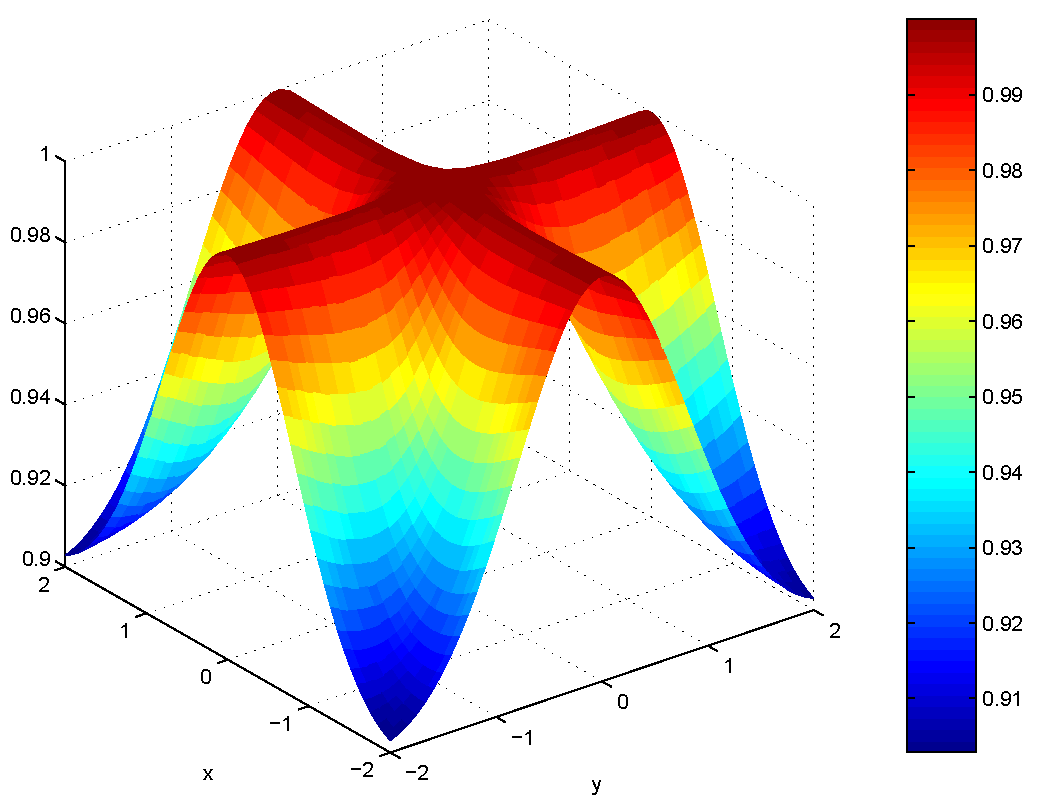
\includegraphics[width=\ScaleIfNeeded]{figuras/grafico-seno.pdf}
\caption{Grafo de $\sen\left(\frac{xy}{x^2+y^2+1}\right)$}
\label{fig:GraficoSeno1}
\end{minipage}
\hfill
\begin{minipage}[t]{.45\textwidth}
\centering
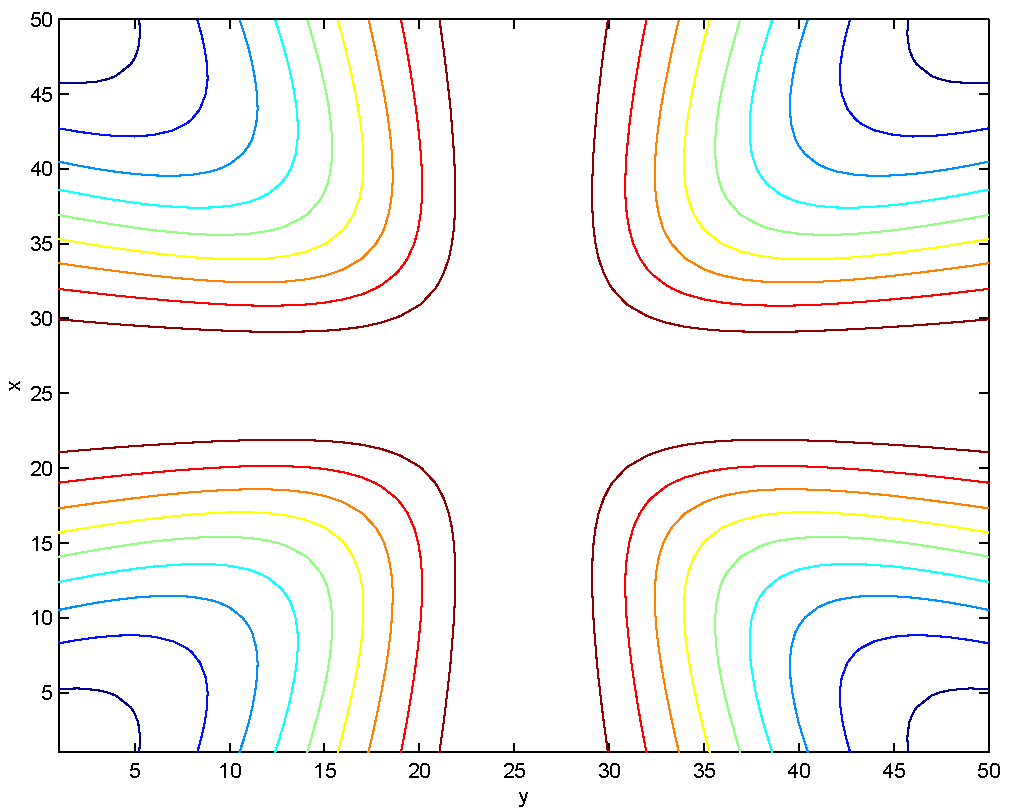
\includegraphics[width=\ScaleIfNeeded]{figuras/curvasdenivel-seno.pdf}
\caption{Curvas de nivel de $\sen\left(\frac{xy}{x^2+y^2+1}\right)$}
\label{fig:GraficoSeno2}
\end{minipage}
\end{figure}
\end{ejemplo}

\section{Conceptos introductorios de topolog\'ia}

La noci\'on de l\'imite\index{L\'imite!de una funci\'on} y continuidad\index{Continuidad!de una funci\'on} de funciones de $\R^n$ en $\R^m$ involucra el car\'acter topol\'ogico de estos espacios, inducido por la norma.

En el estudio de la topolog\'ia de $\R^n$ \index{Topolog\'ia!de $\R^n$}, un rol fundamental es jugado por las
bolas abiertas.
\begin{definicion} Dados $\vec{x}_0\in \R^n$, $r\in \R_+$, llamaremos bola abierta \index{Bola!abierta} de centro en $\vec{x}_0$ y radio $r$ al conjunto
$$B(\vec{x}_0, r)=\{\vec{x}\in \R^n : \|\vec{x}-\vec{x}_0\|<r\}$$
Llamaremos bola cerrada\index{Bola!cerrada} de centro en $\vec{x}_0$ y radio $r$ al conjunto
$$\overline{B}(\vec{x}_0, r)=\{\vec{x}\in \R^n : \|\vec{x}-\vec{x}_0\|\le r\}$$
\end{definicion}

\begin{definicion} Diremos que $A\subseteq \R^n$ es un conjunto abierto\index{Conjunto!abierto} si
$$(\forall \vec{x}_0\in A)( \exists r>0) : B(\vec{x}_0,r)\subseteq A$$
\end{definicion}

\begin{ejemplo}  
$\R^n$ y el conjunto vac\'io\index{Conjunto!vac\'io} $\varnothing$, son 
conjuntos abiertos. A\'un cuando $\R^n$ es obviamente abierto, 
el caso del conjunto vac\'io requiere una reflexi\'on. Si $\varnothing$ no 
es abierto entonces existe $\vec{x}_0\in \varnothing$ para el cual  
$B(\vec{x}_0,r)\cap \R^n \not = \varnothing$, para cada $r>0$. 
Esto es absurdo pues no hay elementos en $\varnothing$.
\end{ejemplo} 

\begin{ejemplo}
El conjunto $A=\{(x,y) : x>1\}$ es un conjunto abierto. En efecto, si
$(x,y)\in A$ entonces $$B\left((x,y), \frac{x-1}{2}\right)\subset A$$
\end{ejemplo} 

\begin{ejemplo}
Si $x_0\in\R$ y $r>0$ entonces $B(x_0,r)$ es un conjunto abierto. En efecto,
si $x\in B(x_0,r)$ entonces $$B\left(x, \frac{(r-\|x-x_0\|)}{2}\right)\subset B(x_0,r)$$ 
Usando la desigualdad triangular 
muestre la veracidad de esta \'ultima afirmaci\'on y haga un dibujo.
\end{ejemplo}

\begin{definicion} 
Diremos que $A\subseteq \R^n$ es un conjunto cerrado\index{Conjunto!cerrado} si $A^C$ es abierto.
\end{definicion}  

\begin{nota}
Los conjuntos $\R^n$ y $\varnothing$ son abiertos y cerrados.
Tambi\'en existen conjuntos que no son abiertos ni cerrados. Ver ejemplo a continuaci\'on.
\end{nota}

\begin{ejemplo} Sean $A=\{\frac{1}{n} :n\in \N\}$ y $B=A\cup\{0\}$. Entonces:
\begin{enumerate}
\item $A$ no es cerrado. En efecto $A^C$ no es abierto, pues $0\in A^C$ y:
$(\forall r>0) \: B(0,r)\not\subseteq A^C.$ Lo anterior pues cualquiera 
sea $r>0$ se tiene que 
$$ 
(\exists n\in \N) \text{ tal que } \frac{1}{n}<r
$$ 
Es decir, $\frac{1}{n} \in B(0,r)$.
\item $A$ no es abierto pues  $1\in A$, pero $(\forall r>0)\: B(x_0,r)\not\subseteq A$.
\item $B$ es cerrado y no es abierto.
\end{enumerate}
\end{ejemplo}

Como en el caso de $\R$ uno puede definir sucesiones de vectores en $\R^n$.
Se trata de una funciones de    $\N \to \R^n$ tales que $k\to \vec{x}_k$. Usualmente
se considera la notaci\'on $\{\vec{x}_k\}_{k\in\N}$. 

\begin{definicion} Una sucesi\'on\index{Sucesi\'on} $\{\vec{x}_k\}_{k\in\N}$ en $\R^n$ se dice sucesi\'on convergente\index{Sucesi\'on!convergente}  a $\vec{x}\in \R^n$ si:
$$(\forall \varepsilon >0)(\exists k_0\in \N)
\::\: \|\vec{x}_k-\vec{x}\|<\varepsilon \: (\forall k\geq k_0)$$
\end{definicion}
En el caso que $\vec{x}\in \R^n$ converge a $\vec{x}$ anotamos $\vec{x}_k\to \vec{x}$ o $\lim_{k\to\infty}\vec{x}_k=\vec{x}$. 
Notamos que la condici\'on $ \|\vec{x}_k-\vec{x}\|<\varepsilon$ es 
equivalente a $\vec{x}_k\in B(\vec{x},\varepsilon).$


Es interesante que uno puede caracterizar los conjuntos cerrados mediante el
uso de sucesiones. En realidad uno podr\'ia describir completamente
la topolog\'ia de 
$\R^n$ usando sucesiones, pero no lo haremos.
\begin{proposicion} $A\subseteq \R^n$ es cerrado si y s\'olo si:
$$
\text{Para toda sucesi\'on } \{\vec{x}_k\}_{k\in\N}\subseteq A : 
(\thinspace (\vec{x}_k\to \vec{x}) \Rightarrow \vec{x}\in A)
$$
\end{proposicion}

\begin{demostracion}
\textcolor{white}{linea en blanco}
\\($\Rightarrow$): Supongamos que $A$ es cerrado. Sea  
$\{\vec{x}_k\}_{k\in\N}\subseteq A$ una sucesi\'on cualquiera tal que
$\displaystyle \lim_{\vec{x}_k\to \vec{x}}\vec{x}_k=\vec{x}$. Queremos demostrar que $\vec{x}\in A$.
Supongamos que no, es decir, que $\vec{x}\in A^C$. Como $A$ es cerrado, existe
$\varepsilon>0$ tal que  $B(\vec{x},\varepsilon)\subset A^C$. 
Por otra parte, de la definici\'on de l\'imite, 
existe $k_0\in\N$ tal que $\vec{x}_k\in B(\vec{x},\varepsilon)$ para todo $k\ge k_0$, lo que
es imposible pues $\vec{x}_k\in A$.

\smallskip

($\Leftarrow$): Para demostrar la rec\'iproca probemos la contrarrec\'iproca.
Es decir, si $A$ no es cerrado entonces existe una sucesi\'on $\{\vec{x}_k\}_{k\in\N}
\subset A$
que converge a $\vec{x}$ y $\vec{x}\not \in A$.

Como $A$ no es cerrado, $A^C$ no es abierto, entonces existe un punto 
$\vec{x}\in A^C$ tal que
$$
\text{Para todo }\varepsilon>0 \text{ se tiene } B(\vec{x},\varepsilon)\cap A\not =\varnothing
$$
Esta proposici\'on nos permite construir una sucesi\'on $\{\vec{x}_k\}\subset A$
de la siguiente manera: para cada $k\in \N$  
tomamos $\varepsilon=\frac{1}{k}$ entonces, como $ B(\vec{x},1/k )\cap A\not 
=\varnothing$, podemos elegir $\vec{x}_k\in B(\vec{x},\frac{1}{k})$ y $\vec{x}_k\in A$. Por 
definici\'on esta sucesi\'on converge a $\vec{x}$, concluyendo la demostraci\'on pues 
$\vec{x}\not \in A$.
\end{demostracion}

Continuando con nuestra discusi\'on sobre la topolog\'ia de $\R^n$ hacemos
algunas nuevas definiciones.

\begin{definicion} Sea $A\subseteq\R^n$. Entonces:
\begin{enumerate}
\item $\vec{x}\in A$ se dice  punto interior\index{Punto!interior} de $A$ si $(\exists\varepsilon>0)\::
\: B(\vec{x},\varepsilon)\subseteq A.$
\item $\vec{x}\in\R^n$  se dice punto adherente\index{Punto!adherente} de $A$ si 
$(\forall\varepsilon>0)\::\: B(\vec{x},\varepsilon)\cap A\neq\varnothing.$
\item $\vec{x}\in\R^n$  se dice punto de acumulaci\'on\index{Punto!de acumulaci\'on} de $A$ si 
$(\forall\varepsilon>0)\::\: (B(\vec{x},\varepsilon)\setminus\{\vec{x}\})\cap A\neq\varnothing.
$
\item $\vec{x}\in\R^n$  se dice punto frontera\index{Punto!frontera} de $A$ si 
$(\forall\varepsilon>0)\::\: B(\vec{x},\varepsilon)\cap A
\neq\varnothing \:\wedge \: B(\vec{x},\varepsilon)\cap A^C\neq\varnothing.
$
\end{enumerate}
\end{definicion}

Observamos que un punto adherente de $A$ no necesita estar en $A$, as\'i mismo
un punto de acumulaci\'on y un punto frontera no necesitan estar en $A$. 

\begin{definicion} Dado $A\subseteq\R^n$ se definen los siguientes
conjuntos:
\begin{enumerate}
\item Interior\index{Interior} de $A$: $\inte{A}=\{\vec{x}\in A : \vec{x} \text{ es punto interior de } A\}$.
\item Adherencia\index{Adherencia} de $A$:  $\adh{A}=\{\vec{x}\in \R^n : \vec{x} \text{ es punto adherente de } A\}$.
\item Derivado\index{Derivado} de $A$: $\der{A}=\{\vec{x}\in\R^n : \vec{x}  \text{ es punto de acumulacion de } A\}$.
\item Frontera\index{Frontera} de $A$: $\partial A=\fr{A}=\{\vec{x}\in\R^n : \vec{x} \text{ es  punto frontera de } A\}$.
\end{enumerate}
\end{definicion}

\begin{nota} 
$\inte{A}\subset A$ y $A\subset \adh{A}$.
\end{nota}

\begin{ejemplo} En $\R$ sea $A=[1,2)\cup \{3\}$. Entonces:
$\der{A}=[1,2]$, 
$\inte{A}=(1,2)$, 
$\adh{A}=[1,2]\cup \{3\}$ y 
$\fr{A}=\{1,2,3\}.$
\end{ejemplo} 

Se obtiene de las definiciones la siguiente proposici\'on:

\begin{proposicion}
$A$ es abierto\index{Conjunto!abierto} si y s\'olo si $A=\inte{A}$ y $A$ es cerrado\index{Conjunto!cerrado} si y s\'olo si $A=\adh{A}$.
\end{proposicion}

\begin{ejemplo} 
Demuestre que $\vec{x}\in \adh{A}$ si y s\'olo si existe una sucesi\'on
$\{\vec{x}_k\}_k\subset A$ tal que $\lim_{k\to\infty}\vec{x}_k=\vec{x}$.

\begin{solucion}\textcolor{white}{linea en blanco}
\\$(\Rightarrow)$ $A$ es cerrado, entonces toda sucesi\'on convergente en $A$ tiene su l\'imite en $A$.
\\Sea la sucesi\'on $\{\vec{x}_k \}, k \in \N:\vec{x}_k \rightarrow \vec{x} \Rightarrow \vec{x} \in A$
$$ \vec{x}_k \rightarrow \vec{x} \Leftrightarrow \forall \varepsilon > 0 \:\exists k_0 \in \N : \forall k \geq k_0 , \vec{x}_k \in B(\vec{x},\varepsilon)$$
Pero $\vec{x}_k \in A$, entonces $\forall \varepsilon > 0$ $B(\vec{x},\varepsilon)\cap A \neq \varnothing \Rightarrow \vec{x} \in \adh{A}$. Sabemos que $A$ es cerrado, lo que en otras palabras es $A=\adh{A}$ lo cual implica que $\vec{x}\in A$.  

\medskip

$(\Leftarrow)$ Toda sucesi\'on convergente del conjunto $A$ tiene su l\'imite en el conjunto, entonces $A$ es cerrado.
\\Supongamos que $\vec{x}\in \adh{A}$, entonces se tiene que 
$$B(\vec{x},\varepsilon)\cap A \neq \varnothing \: \forall \varepsilon > 0$$

Escojamos $\varepsilon = 1/k$, entonces debe tenerse 
$$B(\vec{x},1/k)\cap A \neq \varnothing \: \forall k\in \N$$ 
lo que implica que existe $\vec{x}_k$ perteneciente a $B(\vec{x},1/k)\cap A$ para todo $k\in \N$. Entonces, $\{\vec{x}_k\}$ est\'a en $A$ y $\lim_{k\to\infty}\vec{x}_k=\vec{x}$
\end{solucion}
\end{ejemplo}

Con este ejemplo terminamos esta breve introduci\'on a la
topolog\'ia de $\R^n$ y estamos en condiciones de presentar la noci\'on
de l\'imite de una funci\'on\index{L\'imite!de una funci\'on}.

\section{L\'imites y continuidad}\label{limites}

\begin{definicion} Sea $f:A\subseteq\R^n\to\R^m$ y $\vec{a}\in \der{A}$. Entonces
decimos que $\vec{b}$ es el l\'imite\index{L\'imite!de una funci\'on} de $f$ cuando $\vec{x}$ tiende a $\vec{a}$ y escribimos
$\displaystyle \lim_{\vec{x}\to \vec{a}} f(\vec{x})=\vec{b}$ si
$$
(\forall\varepsilon>0)(\exists\delta>0)\text{ tal que }
(\|\vec{x}-\vec{a}\|\leq \delta)\wedge(\vec{x}\in A)\Rightarrow\|f(\vec{x})-\vec{b}\| \leq \varepsilon
$$ 
\end{definicion}

\begin{nota} 
En la anterior definici\'on pedimos que $\vec{a}\in \der{A}$ para que siempre haya puntos cerca de $\vec{a}$. 
\end{nota}

A continuaci\'on desarrollaremos dos ejemplos en los cuales debemos efectivamente demostrar el valor de un cierto l\'imite. Para ello es necesario dar una f\'ormula que permita determinar $\delta$ dado $\varepsilon$.

\begin{ejemplo} 
Demuestre usando la definici\'on que
$$
\lim_{(x,y)\to (1,1)}(x^2-1)=0
$$
\begin{solucion}
En primer lugar vemos  que a partir de
$$
\|(x,y)-(1,1)\|\leq \delta
$$
se puede deducir directamente que 
\begin{gather}\label{lim1}
|x-1|\leq \delta \text{ e } |y-1|\leq \delta
\text{ y entonces } |x-1|\leq \delta \text{ y } |x|\leq \delta +1 \tag{*}
\end{gather}
Por otro lado 
\begin{gather}\label{lim2}
|f(x)-b|=|x^2-1|=|x-1||x+1| \tag{**}
\end{gather}
As\'i, dado $\varepsilon>0$ podemos elegir $\delta>0$ de modo que 
$$\delta(\delta +2)\leq \varepsilon$$
Entonces, si $\|(x,y)-(1,1)\|\leq \delta$, tenemos \eqref{lim1}, y entonces obtenemos de
\eqref{lim2} que 
$$
\big(|f(x)-b|\leq \delta(\delta+2)\big) \leq \varepsilon
$$
\end{solucion}
\end{ejemplo}

El ejemplo anterior es bastante simple. La dificultad puede aumentar
cuando la funci\'on $f$ es m\'as complicada, por ejemplo si es un
cuociente. 

\begin{ejemplo}
 Demuestre usando la definici\'on que
$$\lim_{(x,y)\to (2,1)}\frac{x^2}{x-y}=4$$
\begin{solucion}
Partimos como en el ejemplo anterior viendo que si 
$$
\|(x,y)-(2,1)\|\leq \delta
$$
entonces se tiene directamente que
\begin{gather}\label{lim3}
|x-2|\leq \delta \text{ e } |y-1|\leq \delta \tag{*}
\end{gather}
Por otro lado, un desarrollo algebraico simple nos lleva a lo siguiente
\begin{gather} \label{lim4}
|f(x)-b|=\left|\frac{x^2}{x-y}-4\right|=\frac{|x^2-4x+4y|}{|x-y|}=
\frac{|(x-2)^2-4(y-1)|}{|x-y|} \tag{**}
\end{gather}
Observamos aqu\'i dos hechos relevantes. Primero, en el numerador tenemos
una expresi\'on que depende esencialmente de $|x-2|$ y $|y-1|$, cantidades 
controladas por $\delta$, seg\'un \eqref{lim3}. Segundo, en el  denominador tenemos 
$|x-y|$, que es una cantidad que podr\'ia anularse si uno no es cuidadoso.

Para tratar este \'ultimo t\'ermino procedemos en una primera etapa encontrando un
valor $\delta_1$ medio, que si bien no nos permitir\'a acotar 
por $\varepsilon$ nos permitir\'a controlar $|x-y|$. El 
denominador no se anula en $(2,1)$,  de aqu\'i vemos que si elegimos
$\delta_1=1/4$, por ejemplo, entonces de \eqref{lim3} podemos concluir que 
\begin{gather}\label{lim5}
|x-y|>\frac{1}{2} \tag{***}
\end{gather}
Suponiendo entonces que \eqref{lim5} se tiene, obtenemos de \eqref{lim3} y \eqref{lim4}  que
$$
|f(x)-b|=
\frac{|(x-2)^2-4(y-1)|}{|x-y|}\leq 2
|(x-2)^2-4
(y-1)|$$
De aqu\'i, usando nuevamente \eqref{lim3} podemos acotar mejor
$$
|f(x)-b|\leq \frac{1}{2}|x-2|+8|y-1|\le 8(|x-2|+|y-1|)
$$ 
Entonces, dado $\varepsilon>0$, podemos elegir $\delta_2=\frac{\varepsilon}{16}.$
Pero debemos asegurarnos que los argumentos anteriores sean siempre v\'alidos
y eso lo logramos si elegimos 
$\delta=
\min\{\frac{1}{2},\frac{\varepsilon}{16}\}$ y se tendr\'a que 
$$\|(x,y)-(2,1)\|\leq \delta\Rightarrow \left|\frac{x^2}{x-y}-4\right|\leq \varepsilon$$
\end{solucion}
\end{ejemplo}

\begin{ejemplo}
Demostrar  que
$$\lim_{(x,y)\to (0,0)}\frac{\sen(x^2+y^2)}{x^2+y^2}=1$$
\begin{solucion}
Del curso de C\'alculo sabemos que
$$\lim_{\alpha\to 0}\frac{\sen(\alpha)}{\alpha}=1$$
Entonces, dado $\varepsilon>0$ existe $\delta_1>0$ tal que 
$$|\alpha|\leq \delta_1\Rightarrow \left|\frac{\sen(\alpha)}{\alpha}-1\right|\leq \varepsilon
$$
Elijamos ahora $\delta=\sqrt{\delta_1}$. Entonces $\|(x,y)-(0,0)\|\leq \delta$ implica
que  $|x^2+y^2|\leq \delta_1$ y entonces
$$\left|\frac{\sen(x^2+y^2)}{x^2+y^2}-1\right|\leq \varepsilon$$
\end{solucion}
\end{ejemplo}

\begin{nota} Notamos que una manera equivalente de escribir la noci\'on 
de l\'imite\index{L\'imite!de una funci\'on} es la siguiente:  para toda bola abierta $B(\vec{b},\varepsilon)$ 
existe una bola abierta $B(\vec{a},\delta)$ tal que
$$\vec{x}\in (B(\vec{a},\delta)\setminus \{\vec{a}\})\cap A\Rightarrow f(\vec{x})\in B(\vec{b},\varepsilon)$$
o equivalentemente
$$f((B(\vec{a},\delta)\setminus \{\vec{a}\})\cap A)\subset  B(\vec{b},\varepsilon)$$
\end{nota}

Ahora vamos a desarrollar el concepto de l\'imite estudiando sus principales
propiedades. En toda esta secci\'on hacemos notar la analog\'ia que se tiene
con el curso de C\'alculo, donde se estudio el concepto de l\'imite y
continuidad para funciones de una variable real. Es sorprendente que la mayor\'ia de las proposiciones que veremos a continuaci\'on tienen una demostraci\'on que
se obtiene de la an\'aloga de C\'alculo reemplazando $|\cdot|$ por $\|\cdot\|$.

\begin{proposicion}{\rm (Unicidad del l\'imite)\index{L\'imite!unicidad}} 
\\Sea $f:A\subseteq \R^n\to\R^m$ y 
$\vec{a}\in \der{A}$. Si 
$$\lim_{\vec{x}\to \vec{a}}f(\vec{x})=\vec{b}_1 \text{ y } \lim_{\vec{x}\to \vec{a}}f(\vec{x})=\vec{b}_2$$
Entonces $\vec{b}_1 = \vec{b}_2$.
\end{proposicion}

\begin{demostracion}
Por hip\'otesis, dado $\varepsilon>0$ existen $\delta_1>0$ y
$\delta_2>0$ tales que
$$(\|\vec{x}-\vec{a}\|\leq \delta_1 \:\wedge \: \vec{x}\in A)\Rightarrow \|f(\vec{x})-\vec{b}_1\|\leq \varepsilon$$
$$(\|\vec{x}-\vec{a}\|\leq \delta_2 \:\wedge \: \vec{x}\in A)\Rightarrow \|f(\vec{x})-\vec{b}_2\|\leq \varepsilon$$
Entonces, si $\|\vec{x}-\vec{a}\|\leq \min\{\delta_1,\delta_2\}$ se tendr\'a que
$$\|\vec{b}_1-\vec{b}_2\|\leq \|(f(\vec{x})-\vec{b}_1)-(f(\vec{x})-\vec{b}_2)\|\leq \|f(\vec{x})-\vec{b}_1\|+\|f(\vec{x})-\vec{b}_2\| \leq 2\varepsilon$$
Como $\varepsilon$ puede ser arbitrariamente peque\~no, debemos tener que $\vec{b}_1=\vec{b}_2$.
\end{demostracion}

La siguiente proposici\'on es muy \'util para estudiar la existencia de
un determinado l\'imite. Se usa principalmente para mostrar que una cierta funci\'on no tiene l\'imite.

\begin{proposicion} 
Sea $f:A\subseteq\R^n\to \R^m$ y $\vec{a}\in \der{A}$ tal que $\displaystyle \lim_{\vec{x}\to \vec{a}}f(\vec{x})=\vec{b}$. Entonces para todo $B\subseteq A$ tal que $\vec{a}\in der(B)$ se tiene que
$$\lim_{\vec{x}\to \vec{a}}f|_B(\vec{x})=\vec{b}$$
\end{proposicion}

\begin{demostracion}
\emph{Tarea}.
\end{demostracion}

La contrarrec\'iproca nos da el siguiente corolario
\begin{corolario} Sea $f:A\subseteq\R^n\to\R^m$, $\vec{a}\in \der{A}$ y 
$B_1,B_2\subseteq A,$ de manera que $\vec{a}\in der(B_1)\cap der(B_2)$. 
Si uno de los l\'imites $\displaystyle \lim_{\vec{x}\to \vec{a}}f|_{B_1}(\vec{x})$ \'o $\displaystyle \lim_{\vec{x}\to \vec{a}}f|_{B_2}(\vec{x})$
no existe o si $\displaystyle \lim_{\vec{x}\to \vec{a}}f|_{B_1}(\vec{x})\neq \displaystyle \lim_{\vec{x}\to \vec{a}}f|_{B_2}(\vec{x})$ entonces el l\'imite
$$\lim_{\vec{x}\to \vec{a}}f(\vec{x})=\vec{b}$$
no existe.
\end{corolario}

\begin{ejemplo} 
Se trata de estudiar el siguiente l\'imite 
$$
\lim_{(x,y)\to (0,0)}\frac{x}{x+y}
$$
\begin{solucion} 
Notemos en primer lugar que $f(0,0)$ no est\'a definida, sin embargo esto no tiene
importancia alguna. Lo que s\'i importa es que $(0,0)\in der(\R^2\setminus \{(0,0)\})$.
Si consideramos los conjuntos $A=\{(0,y): y\neq 0\}$ y  $B=\{(x,0):x\neq 0\}$ entonces  tenemos  que
$$\lim_{(x,y)\to (0,0)}f|_A(x,y)=0 \text{ y } \lim_{(x,y)\to (0,0)}f|_B(x,y)=1$$
Concluimos entonces que el
l\'imite bajo estudio  no existe, en virtud del corolario.
\end{solucion}
\end{ejemplo}   

\begin{nota} En los ejemplos anteriores hemos considerado solamente
funciones a valores reales, es decir,  con espacio de llegada $\R$. Esto queda 
justificado en la siguiente proposici\'on.
\end{nota}

\begin{proposicion}\label{proposicion18}
Sea $f:A\subseteq\R^n\to\R^m$. Entonces:
$$\lim_{\vec{x}\to \vec{a}}f(\vec{x})=\vec{b}\quad \Leftrightarrow \quad (\forall i=1,\ldots,m)\lim_{\vec{x}\to \vec{a}}f_i(\vec{x})=b_i$$
Aqu\'i $f_i$ es la i-\'esima funci\'on coordenada\index{Funci\'on!coordenada} y $b_i$ is la i-\'esima coordenada de $\vec{b}$.
\end{proposicion}

\begin{demostracion}
\textcolor{white}{linea en blanco}
\\($\Rightarrow$): \emph{Tarea}.

($\Leftarrow$): Dado $\varepsilon>0$, por hip\'otesis existe $\delta_i>0$ tal que 
$\|\vec{x}-\vec{a}\|\leq \delta_i$ y $\vec{x}\in A$ implica que $|f_i(\vec{x})-b_i|\leq \varepsilon/\sqrt{m}$, para cualquier
$i=1,2,\ldots,m$. Entonces, si elegimos $\delta=\min\{\delta_1, \ldots,\delta_m\}$. tenemos que si $\|\vec{x}-\vec{a}\|\leq \delta$ y $\vec{x}\in A$ implica
$$
\sum_{i=1}^m(f_i(\vec{x})-b_i)^2<m\cdot\frac{\varepsilon^2}{m}=\varepsilon^2
$$
de donde $\|f(\vec{x})-\vec{b}\|\leq\varepsilon$.
\end{demostracion}

Los siguientes tres teoremas resumen las propiedades importantes de los l\'imites.

%\begin{teorema}\label{teolimites1-antiguo}
%Sean $f, g:A\subseteq\R^n\to\R^m$, 
% $\vec{x}_0\in \der{A}$, $\vec{b},\vec{d}\in\R^m$ y $c\in\R$. Entonces:
%\begin{enumerate}
%\item ${\lim_{\vec{x}\to \vec{x}_0}f(\vec{x})=\vec{b}}$ $\Rightarrow$ ${\lim_{\vec{x}\to \vec{x}_0}cf(\vec{x})=c\vec{b}}$
%\item $\lim_{\vec{x}\to \vec{x}_0}f(\vec{x})=\vec{b}$ y $\lim_{\vec{x}\to \vec{x}_0}g(\vec{x})=\vec{d}$ $\Rightarrow$
%	\begin{enumerate}
%	\item $\lim_{\vec{x}\to \vec{x}_0}(f(\vec{x})+g(\vec{x}))=\vec{b}+\vec{d}$
%	\item $\lim_{\vec{x}\to \vec{x}_0}f(\vec{x})\cdot g(\vec{x})=\vec{b}\cdot \vec{d}$
%	\end{enumerate}
%\item $m=1$ y $\lim_{\vec{x}\to \vec{x}_0}f(\vec{x})=b\neq 0$ $\Rightarrow$ $\lim_{\vec{x}\to \vec{x}_0}\frac{1}{f(\vec{x})}=\frac{1}{b}$
%\end{enumerate}
%\end{teorema}  

%\begin{demostracion}
%Haremos la demostraci\'on de $\lim_{\vec{x}\to \vec{x}_0}(f(\vec{x})+g(\vec{x}))=\vec{b}+\vec{d}$. Las dem\'as propiedades quedan de \emph{tarea}. 

%Usando la desigualdad triangular y la de Cauchy-Schwarz obtenemos directamente
%\begin{eqnarray*}
%\|f(\vec{x})\cdot g(\vec{x})-\vec{b}\cdot \vec{d}\|& =&
%\|f(\vec{x})\cdot 
%(g(\vec{x})-d)+d\cdot (f(\vec{x})-b)\|\cr
%&\leq&\|f(\vec{x})\|\,\|g(\vec{x})-d\|+\|d\|\,\|f(\vec{x})-b\|.
%\end{eqnarray*}
%Usando la hip\'otesis,  dado $\varepsilon>0$ tenemos que existe $\delta>0$ tal que 
%$\vec{x}\in A$ y $ 0< \|\vec{x}-\vec{x}_0\|<\delta$ implica que 
%$$\|f(\vec{x})-\vec{b}\|<{\varepsilon} \text{ y } \|g(\vec{x})-\vec{d}\|<{\varepsilon}$$
%Notamos que de aqu\'i se deduce que $\|f(\vec{x})\|<\varepsilon+\|\vec{b}\|.$ Por lo tanto
%$$
%\|f(\vec{x})\cdot g(\vec{x})-\vec{b}\cdot \vec{d}\|<(\varepsilon+\|\vec{b}\|+\|\vec{d}\|)\varepsilon
%$$
%completando la demostraci\'on.
%\end{demostracion}

%\begin{nota} En rigor, en la demostraci\'on anterior falta un paso, el cual
%se puede siempre omitir cuando hay experiencia:
%\\Dado $\varepsilon>0$ elegimos $\sigma>0$ tal que $(\sigma+\|b\|+\|d\|)\sigma<\varepsilon.$ Con este valor de $\sigma>0$ invocamos la hip\'otesis para elegir $\delta>0$ de modo que $\vec{x}\in A$ y $ 0< \|\vec{x}-\vec{x}_0\|<\delta$ implica que
%$$\|f(\vec{x})-b\|<{\sigma} \text{ y } \|g(\vec{x})-d\|<{\sigma}$$
%\end{nota} 

\begin{teorema}\label{teolimites1}
Sean $f,g:A\subseteq\R^n\to\R^m$ y $\vec{a}\in \der{A}$. Si existen los l\'imites $\displaystyle \lim_{\vec{x}\to \vec{a}} f(\vec{x}) = \vec{b}_1$ y $\displaystyle \lim_{\vec{x}\to \vec{a}} g(\vec{x}) = \vec{b}_2$, entonces los siguientes l\'imites existen y pueden calcularse como sigue:
\begin{align}
\lim_{\vec{x} \to \vec{a}} (f+g)(\vec{x}) &= \lim_{\vec{x} \to \vec{a}} f(\vec{x}) + \lim_{\vec{x} \to \vec{a}} g(\vec{x}) \\
\intertext{Si $\lambda \in \R$,}
\lim_{\vec{x} \to \vec{a}} (\lambda f)(\vec{x}) &= \lambda \lim_{\vec{x} \to \vec{a}} f(\vec{x})
\end{align}
\end{teorema}

\begin{demostracion} Demostraremos una a una las propiedades:
\begin{enumerate}
\item Dado $\varepsilon > 0$, como $f$ y $g$ tienen l\'imite en $\vec{a}$, existen $\delta_1,\delta_2 > 0$ tales que
\begin{align*}
\vec{x} \in A, \|\vec{x}-\vec{a}\| \leq \delta_1 \:\Rightarrow\: \|f(\vec{x}-f(\vec{a}))\| \leq \frac{\varepsilon}{2} \\
\vec{x} \in A, \|\vec{x}-\vec{a}\| \leq \delta_2 \:\Rightarrow\: \|g(\vec{x})-g(\vec{a})\| \leq \frac{\varepsilon}{2}
\end{align*}
Definiendo $\delta = \min\{\delta_1,\delta_2\}$ se obtiene:
\begin{align*}
\vec{x}\in A,\:\|\vec{x}-\vec{a}\| \leq \delta \:\Rightarrow\: & \|(f+g)(\vec{x})-(f+g)(\vec{a})\| \leq \\
& \|f(\vec{x})-f(\vec{a})\| + \|g(\vec{x})-g(\vec{a})\| \leq \frac{\varepsilon}{2} + \frac{\varepsilon}{2} = \varepsilon
\end{align*}

\item Si $\lambda= 0$ se concluye la demostraci\'on. Si $\lambda \neq 0$, dado $\varepsilon > 0$ como $f$ tiene l\'imite en $\vec{a}$, existe $\delta > 0$ tal que
$$\vec{x}\in A,\: \|\vec{x}-\vec{a}\| \leq \delta \:\Rightarrow\: \|f(\vec{x})-f(\vec{a})\| \leq \frac{\varepsilon}{|\lambda|}$$
lo que es equivalente a $\|\lambda f(\vec{x})- \lambda f(\vec{a})\| \leq \varepsilon$ lo que concluye la demostraci\'on.
\end{enumerate}
\end{demostracion}

\begin{teorema}\label{teolimites1-1}
Sean $f:A\subseteq \R^n \to \R^m$ y $g:f(A)\subseteq \R^m \to \R^p$. Si existen los l\'imites $\displaystyle \lim_{\substack{\vec{x}\to \vec{a}\\\vec{x}\in A}} f(\vec{x}) = \vec{b}$ y $\displaystyle \lim_{\substack{\vec{y}\to \vec{b}\\\vec{y}\in f(A)}} g(\vec{y}) = \vec{c}$, entonces existe el l\'imite 
\begin{equation}
\lim_{\substack{\vec{x}\to \vec{a}\\ \vec{x}\in A}} (g\circ f)(\vec{x}) = \vec{c}
\end{equation}
\end{teorema}

\begin{demostracion}
Dado $\varepsilon > 0$, como el l\'imite de $g$ en $f(\vec{a})$ existe, entonces existe un valor $\eta > 0$ tal que 
$$\|\vec{y}-f(\vec{a})\| \leq \eta \:\Rightarrow\: \|g(\vec{y})-g(f(\vec{a}))\| \leq \varepsilon $$
y como el l\'imite de $f$ en $\vec{a}$ existe, entonces existe un valor $\delta > 0$ tal que
$$\|\vec{x}-\vec{a}\|\leq \delta \:\Rightarrow\: \|f(\vec{x})-f(\vec{a})\|\leq \eta$$ 
De estos dos resultados se concluye
$$\|\vec{x}-\vec{a}\| \leq \delta \:\Rightarrow\: \|g(f(\vec{x}))-g(f(\vec{a}))\|\leq \varepsilon$$
por lo que $g\circ f$ tiene l\'imite en $\vec{a}$.
\end{demostracion}

\begin{teorema}\label{teolimites1-2}
Sean $f,g:A\subseteq \R^n \to \R$. Si existen los l\'imites $\displaystyle \lim_{\vec{x}\to \vec{a}} f(\vec{x}) = b_1$ y $\displaystyle \lim_{\vec{x}\to \vec{a}} g(\vec{x}) = b_2$, entonces los siguientes l\'imites existen y pueden calcularse como sigue:
\begin{align}
\lim_{\vec{x} \to \vec{a}} (f\cdot g)(\vec{x}) &= \lim_{\vec{x} \to \vec{a}} f(\vec{x}) \cdot \lim_{\vec{x} \to \vec{a}} g(\vec{x}) \\
\intertext{Si $f(\vec{a})\neq 0$}
\lim_{\vec{x} \to \vec{a}} \left(\frac{1}{f}\right)(\vec{x}) &=  \frac{1}{\displaystyle\lim_{\vec{x} \to \vec{a}} f(\vec{x})}
\end{align}
\end{teorema}

\begin{demostracion}
Demostraremos una a una las propiedades y utilizaremos los dos teoremas anteriores. 
\begin{enumerate}
\item Como $(f\cdot g)(\vec{x}) = \frac{1}{2}[(f+g)^2-f^2-g^2](\vec{x})$, para demostrar la existencia del l\'imite de $f\cdot g$ en $\vec{a}$, la demostraci\'on se reduce al hecho de que el cuadrado de una funci\'on cuyo l\'imite existe en $\vec{a}$ tambi\'en tiene l\'imite en $\vec{a}$. 

Debemos demostrar $f^2$ tiene l\'imite en $\vec{a}$. Como $f^2$ es la composici\'on de $f:A\subseteq \R^n \to \R$ con $g: \R \to \R$ definida por $g(y)=y^2$, y como el l\'imite de ambas funciones existe en $\vec{a}$ y $f(\vec{a})$ respectivamente, $f^2$ tiene l\'imite en $\vec{a}$.

\item Siguiendo el desarrollo de la parte anterior, tenemos que $1/f$ es la composici\'on de $f:A\subseteq \R^n \to \R$ con $g:\R\setminus \{0\} \to \R$, definida por $g(y)=1/y$, cuyos l\'imites existen en $\vec{a}$ y $f(\vec{a})$ respectivamente.
\end{enumerate}
\end{demostracion}

\subsection{Continuidad de funciones de \texorpdfstring{$\R^n$}{Rn} en \texorpdfstring{$\R^m$}{Rm}}
Ahora que hemos estudiado el concepto de l\'imite estamos 
preparados para introducir el concepto de continuidad de una funci\'on\index{Continuidad!de una funci\'on}.

\begin{definicion} Sea $f:A\subseteq\R^n\to\R^m$ y sea $\vec{y}\in A$. 
Decimos que $f$ es continua\index{Funci\'on!continua} en $\vec{y}$ si:
$$(\forall\varepsilon>0)(\exists\delta>0) \text{ tal que } [\vec{x}\in A \:\wedge \: \|\vec{x}-\vec{y}\|\leq \delta] \:\Rightarrow\: \|f(\vec{x})-f(\vec{y})\|\leq \varepsilon$$
o equivalentemente
$$(\forall\varepsilon>0)(\exists\delta>0) \text{ tal que } f(B(\vec{y},\delta)\cap A)\subset B(f(\vec{y}),\varepsilon)
$$
\end{definicion}

\begin{definicion} Sea $f:A\subseteq\R^n\to\R^m$. Decimos que $f$ es continua\index{Funci\'on!continua} en $A$ si:
$$(\forall \vec{x}\in A)(\forall\varepsilon>0)(\exists\delta>0) \text{ tal que } [\vec{y} \in A \:\wedge \: \|\vec{x}-\vec{y} \|\leq \delta] \:\Rightarrow\: \|f(\vec{x})-f(\vec{y})\|\leq \varepsilon$$
\end{definicion}

\begin{nota}
Si $\vec{x}_0\in A$ es un punto aislado\index{Punto!aislado} de A, es decir, $\vec{x}_0\in A\setminus \der{A}$ 
entonces $f$ es obviamente continua en $\vec{x}_0$.

Si $\vec{x}_0\in \der{A}$ entonces $f$ es continua en $\vec{x}_0$ si y s\'olo si
$$\lim_{\vec{x}\to \vec{x}_0}f(\vec{x})=f(\vec{x}_0)$$
\end{nota}

Como consecuencia de la observaci\'on anterior y de la proposici\'on \ref{proposicion18} se tiene que $f:A\subseteq\R^n\to\R^m$ es continua en $\vec{x}_0\in A$ si y s\'olo si $f_i$ es continua en $\vec{x}_0,$ para todo $i=1,\ldots,m.$

Como consecuencia de los teoremas \ref{teolimites1}, \ref{teolimites1-1} y \ref{teolimites1-2} tenemos tambi\'en tres resultados sobre funciones continuas cuya demostraci\'on es an\'aloga a lo que ya vimos sobre l\'imites.

\begin{teorema}\label{teolimites2} 
Sean $f,g:A\subseteq\R^n\to\R^m$, $\vec{x}_0\in A$ y $\lambda\in\R$. Entonces:
\begin{enumerate}
\item $f$ continua en $\vec{x}_0$ implica $\lambda f$ continua en $\vec{x}_0$.
\item $f$ y $g$ continuas en $\vec{x}_0$ implica $f+g$ continua en $\vec{x}_0$.
\end{enumerate}
\end{teorema} 

\begin{demostracion}
\emph{Tarea.}
\end{demostracion}

\begin{teorema}\label{teolimites2-1} 
Sean $f:A\subseteq\R^n\to\R^m$, $g:B\subseteq \R^m \to \R^p$, con $f(A)\subseteq B$ y $\vec{x}_0\in A$. Entonces $f$ continua en $\vec{x}_0$ y $g$ continua en $f(\vec{x}_0)$ implica $g\circ f$ continua en $\vec{x}_0$.
\end{teorema} 

\begin{demostracion} 
Sea $\varepsilon>0.$ Como $g$ es continua en 
$f(\vec{x}_0)$ existe $\delta>0$ tal que: 
$$ \vec{y}\in B,\:\|\vec{y}-f(\vec{x}_0)\|\leq \delta \:\Rightarrow\: \|g(\vec{y})-g(f(\vec{x}_0))\|\leq \varepsilon$$
Por otro lado, de la continuidad de $f$ en $\vec{x}_0$ sabemos que existe 
$\eta>0$ tal que:
$$\vec{x}\in A,\: \|\vec{x}-\vec{x}_0\|\leq \eta\:\Rightarrow\:\|f(\vec{x})-f(\vec{x}_0)\|\leq \delta$$
Juntando estas dos proposiciones y tomando $\vec{y}=f(\vec{x})$ se tiene que existe $\eta>0$
tal que
\begin{eqnarray*}
& & \vec{x}\in A,\: \|\vec{x}-\vec{x}_0\|\leq \eta\:\Rightarrow\: f(\vec{x})\in B,\: 
\|f(\vec{x})-f(\vec{x}_0)\|\leq \delta \cr
& & \Rightarrow\:\|g(f(\vec{x}))-g(f(\vec{x}_0))\|\leq \varepsilon
\end{eqnarray*}
Es decir:$$\|\vec{x}-\vec{x}_0\|\leq \eta\:\Rightarrow\:\|(g\circ f)(\vec{x})-(g\circ f)(\vec{x}_0)\|\leq \varepsilon $$
\end{demostracion}

\begin{teorema}\label{teolimites2-2}
Sean $f,g:A\subseteq\R^n\to\R$ y $\vec{x}_0\in A$. Entonces $f$ y $g$ continuas en $\vec{x}_0$ implica $f\cdot g$ continua en $\vec{x}_0$. Agregando el supuesto $f(\vec{x}_0)\neq 0$, $f$ y $g$ continuas en $\vec{x}_0$ implica $\frac{1}{f(\vec{x})}$ continua en $\vec{x}_0$.
\end{teorema}

\begin{demostracion}
\emph{Tarea.}
\end{demostracion}

\begin{ejemplo} 
La funci\'on $f(x,y)=(\frac{x^2}{1+y^2},x+y,y\cdot \sen(x))$ es 
continua en todo punto de $\R^2$.

\begin{solucion}
En efecto, sus tres componentes son continuas en todo $\R^2$:

$f_1(x,y)=\frac{x^2}{1+y^2}$ lo es pues $f(x)=x^2$ lo es, al igual que 
$g(y)=1+y^2$ la cual adem\'as no se anula. Entonces, por el teorema anterior 
$\frac{1}{g(y)}=\frac{1}{1+y^2}$ tambi\'en es continua, y 
nuevamente por el teorema anterior $x^2\frac{1}{1+y^2}$ es continua.

$f_2(x,y)=x+y$ es evidentemente continua pues $f(x)=x$ e $g(y)=y$ son continuas y la suma de continuas es continua por el teorema anterior.

$f_3(x)=\sen(x)$ es continua, $g(y)=y$ tambi\'en lo es, luego por el teorema anterior $y\cdot \sen(x)$ es continua.

La idea es que con la ayuda de los teoremas \ref{teolimites2}, \ref{teolimites2-1} y \ref{teolimites2-2} podamos determinar por inspecci\'on cuando una funci\'on es continua, por ser una combinaci\'on de funciones continuas conocidas.
\end{solucion}
\end{ejemplo}

\begin{ejemplo} 
$f(x,y,z,t)=\sen(t(x^2+y^2+z^2))$ es continua en todo punto de $\R^4$.
\end{ejemplo}

%En la l\'inea del teorema \ref{teolimites2}, tenemos el teorema de la composici\'on de
%funciones continuas.
%\begin{teorema} Sean $f:A\subseteq\R^n\to\R^m$ y $g:B\subseteq\R^m\to\R^p$ tales que %$f(A)\subseteq B$. Si $f$ es continua\index{Funci\'on!continua} en 
%$\vec{x}_0\in A$ y $g$ es continua en $f(\vec{x}_0)\in B$ entonces $g\circ %f$\index{Composici\'on!de funciones continuas} es continua en $\vec{x}_0$.
%\end{teorema}

%\begin{demostracion} 
%Sea $\varepsilon>0.$ Como $g$ es continua en 
%$f(\vec{x}_0)$ existe $\delta>0$ tal que: 
%$$ \vec{y}\in B,\:\|\vec{y}-f(\vec{x}_0)\|<\delta \:\Rightarrow\: \|g(\vec{y})-g(f(\vec{x}_0))\|<\varepsilon$$
%Por otro lado, de la continuidad de $f$ en $\vec{x}_0$ sabemos que existe 
%$\delta'>0$ tal que:
%$$\vec{x}\in A,\: \|\vec{x}-\vec{x}_0\|<\delta'\:\Rightarrow\:\|f(\vec{x})-f(\vec{x}_0)\|<\delta$$
%Juntando estas dos proposiciones y tomando $y=f(\vec{x})$ se tiene que existe $\delta'>0$
%tal que
%\begin{eqnarray*}
%& & \vec{x}\in A,\: \|\vec{x}-\vec{x}_0\|<\delta'\:\Rightarrow\: f(\vec{x})\in B,\: 
%\|f(\vec{x})-f(\vec{x}_0)\|<\delta \cr
%& & \Rightarrow\:\|g(f(\vec{x}))-g(f(\vec{x}_0))\|<\varepsilon
%\end{eqnarray*}
%Es decir:$$\|\vec{x}-\vec{x}_0\|<\delta'\:\Rightarrow\:\|g\circ f(\vec{x})-g\circ f(\vec{x}_0)\|<
%\varepsilon $$
%\end{demostracion}

\begin{definicion} 
Diremos que $A\subseteq\R^n$ es una vecindad\index{Vecindad} de $\vec{x}_0\in\R^n$ si $\vec{x}_0\in A$ y $A$ es abierto.
\end{definicion}

La siguiente proposici\'on da una caracterizaci\'on de la continuidad en t\'erminos de vecindades. Notar que la bola abierta $B(\vec{x},r)$ es una vecindad de $\vec{x}$.

\begin{proposicion} $f:A\subseteq\R^n\to\R^m$ es continua en $\vec{x}_0\in\R^n$ si y s\'olo si para toda vecindad $U\subset \R^n$ de $f(\vec{x}_0)$ existe una vecindad $V\subset\R^n)$ de $\vec{x}_0$ tal que $f(V\cap A)\subset U.$
\end{proposicion}

\begin{demostracion} 
\textcolor{white}{linea en blanco}
\\($\Rightarrow$): Sea $U$ una vecindad de $f(\vec{x}_0)$. Entonces
existe  $\varepsilon>0$ tal que $B(f(\vec{x}_0),\varepsilon)\subset U$. 
Usando ahora la continuidad de $f$ en $\vec{x}_0$,  para este $\varepsilon>0$ 
existe $\delta>0$ tal que
$$\|\vec{x}-\vec{x}_0\|\leq \delta \text{ y }
\vec{x}\in A\Rightarrow\|f(\vec{x})-f(\vec{x}_0)\|\leq \varepsilon
$$
Es decir
$$\vec{x}\in B(\vec{x}_0,\delta) \text{ y } \vec{x}\in A\Rightarrow\: f(\vec{x})\in B(f(\vec{x}_0),\varepsilon)
$$
Si definimos $V=B(\vec{x}_0,\delta)$, que  es una vecindad de $\vec{x}_0$, obtenemos de aqu\'i que 
$$f(B(\vec{x}_0,\delta)\cap A)=f(V\cap A)\subset U$$

\smallskip

($\Leftarrow$): Esta implicaci\'on queda de \emph{tarea}.
 \end{demostracion}

\section{Diferenciabilidad de funciones de \texorpdfstring{$\R^n$}{Rn} a \texorpdfstring{$\R^m$}{Rm}}\label{1.4}

Consideremos $f:A\subseteq\R^n\to\R$ y $\vec{x}=(x_1,\ldots,x_j,\ldots,x_n)\in A$,
donde el conjunto $A$ se supone abierto a fin de evitar complicaciones con cualquier noci\'on similar a la de derivadas laterales como suele hacerse en el c\'alculo de una variable. Para $1\le j\le n$ fijo, definimos 
la funci\'on:
\begin{eqnarray*}
f: \R & \rightarrow & \R \\
h 	  & \mapsto     & f( \vec{x}+h\vec{e}_j )
\end{eqnarray*}
donde $\vec{e}_j$ es el elemento $j$-\'esimo de la 
base can\'onica de $\R^n$. Notamos que 
$$\vec{x}+h\vec{e}_j=(x_1,\ldots,x_{j-1},h+x_j,x_{j+1},\ldots,x_n)$$ 
A esta funci\'on, siendo de $\R$ en $\R$, le podemos aplicar la
teor\'ia de diferenciabilidad desarrollada en el curso de C\'alculo. 
%Aqu\'i las variables  $x_1,\ldots,x_{j-1},x_{j+1},\ldots,x_n$ se mantienen 
%fijas. 
\begin{definicion} Llamaremos derivada parcial \index{Derivada!parcial} de $f$ con respecto a 
$x_j$ en $\vec{x}\in\R^n$ a
$$\frac{\partial f}{\partial x_j}(\vec{x})=\lim_{h\to 0}\frac{f( \vec{x}+h\vec{e}_j)
-f(\vec{x})}{h}$$
si dicho l\'imite existe.
Cuando la derivada parcial de $f$ con respecto a $x_j$ existe en todo punto de 
$A$, entonces ella define una funci\'on 
$$\frac{\partial f}{\partial x_j}:
A\subseteq\R^n\to\R$$
\end{definicion}

\begin{nota} 
Como una derivada parcial es una derivada de una funci\'on de $\R$ en $\R$, uno puede usar todas las reglas de derivaci\'on estudiadas en C\'alculo.
\end{nota}

\begin{ejemplo} 
Calcular la derivada parcial de la funci\'on $f$ con respecto a $x$ para 
$$f(x,y)=x^4 y+\sen(xy)$$

\begin{solucion}
Haciendo uso de la observaci\'on anterior tendremos que
$$\dfx(x,y)=4x^3 y+\cos(xy)y$$
\end{solucion}
\end{ejemplo}

\begin{ejemplo}  
Calcular la derivada parcial de la funci\'on $f$ con respecto a $x$ para
$f(x,y)=\frac{xy}{\sqrt{x^2+y^2}}$.
\end{ejemplo}

\begin{solucion}
Para esto notamos que si $(x,y)\neq(0,0)$ entonces 
$$\dfx(x,y)=\frac{y^3}{(x^2+y^2)^{3/2}}$$
Si definimos $f(0,0)=0$ entonces podemos calcular tambi\'en la derivada parcial
de $f$ con respecto a $x$ en $(0,0)$. Aqu\'i usamos la definici\'on
$$\dfx(0,0)=\lim_{h\to 0}\frac{f(h,0)-f(0,0)}{h}=\lim_{h\to 0}\frac{0}{h}=0$$
\end{solucion}

En la noci\'on de diferenciabilidad hay dos aspectos a considerar:
el aspecto anal\'itico y el aspecto
 geom\'etrico.
Parece tentador definir una funci\'on diferenciable en un punto como una  
funci\'on
que posee  todas sus derivadas parciales en dicho punto. Sin embargo 
esta condici\'on no es suficiente para producir una buena definici\'on, 
 pues nos gustar\'ia que al menos se cumplan las siguientes
propiedades:
\begin{enumerate}
\item Si $f$ es diferenciable en un punto entonces es posible definir un plano 
tangente al grafo de la funci\'on en dicho punto. Este es el criterio
geom\'etrico.
\item La composici\'on de funciones diferenciables 
es diferenciable. Este ser\'ia un criterio  anal\'itico.
\end{enumerate}

\begin{ejemplo}\label{diferenciabilidad-1} 
El siguiente ejempo ilustra las ideas anteriores.
Consideremos la funci\'on definida por $f(x,y)=x^{1/3}y^{1/3}$. 
Calculando las derivadas parciales por definici\'on obtenemos que estas existen 
y son
$$\dfx(0,0)=\dfy(0,0)=0$$  
Uno esperar\'ia que el plano tangente a la funci\'on $f$
en el punto $(0,0,0)$ estuviera dado por la ecuaci\'on $z=0$, para ser consecuentes
con el valor de las derivadas parciales de $f$ en el $(0,0)$. Sin embargo,
este plano no puede ser tangente al  grafo de la funci\'on en $(0,0)$, 
pues sobre la recta $y=x$ el grafo de $f$ tiene pendiente infinita en el origen.

Por otro lado, $g:\R\to\R^2$ definida por $g(x)=(x,x)$ 
es diferenciable en cero con $g'_1(0)=g'_2(0)=1$, pero 
$f\circ g(x)=x^{2/3}$ no es diferenciable en 0.
\end{ejemplo}

Concluimos de este ejemplo que la noci\'on de diferenciabilidad debe 
involucrar algo m\'as que la sola existencia de las 
derivadas parciales en el punto.

Veamos ahora el aspecto geom\'etrico en $\R^2$ para motivar 
la definici\'on en general.
%\\Notemos antes que la derivada parcial con respecto a $x_j$ de una
% funci\'on $f$ en un punto $(x_1,\ldots,x_n)$ es la pendiente 
%o el crecimiento de la funci\'on en la direcci\'on 
%unitaria j-\'esima en el punto $(x_1,\ldots,x_n)$.  
Supongamos que queremos ajustar un plano tangente al grafo de $f:\R^2\to\R$ 
en el punto $(x_0,y_0,f(x_0,y_0))\in G(f)$. Es decir queremos 
encontrar un plano en $\R^3$ que pase por el punto y que 
tenga la misma inclinaci\'on que el grafo de $f$ en el punto. 
Para 
esto consideremos  un plano gen\'erico $z=a+bx+cy$ y deduzcamos de 
las condiciones que mencionamos antes el valor de las constantes $a,b$ y $c$. 
En primer lugar queremos que $(x_0,y_0,z_0)$ pertenezca al plano tangente, entonces
$$f(x_0,y_0)=z_0=a+bx_0+cy_0$$
Fijando la variable $x_0$ se deber\'ia tener que las recta $z=a+bx_0+cy$ debe
ser tangente al grafo de $z=f(x_0,y)$ en el punto $y_0$. Esto implica que
$$\dfx(x_0,y_0)=b$$
De manera an\'aloga
$$\dfy(x_0,y_0)=c$$
Es decir, el plano buscado es
$$z=f(x_0,y_0)+\dfx(x_0,y_0)(x-x_0)+\dfy(x_0,y_0)(y-y_0)$$  
 
\begin{definicion} Sea $f:A\subseteq\R^2\to\R$, $A$ abierto 
y $(x_0,y_0)\in A$. Decimos que $f$ es diferenciable\index{Funci\'on!diferenciable} en $(x_0,y_0)$ si 
existen las derivadas parciales $\dfx(x_0,y_0)$ y $\dfy(x_0,y_0)$  y el l\'imite
\begin{equation*}
\lim_{(x,y)\to (x_0,y_0)}\frac{|f(x,y)-f(x_0,y_0)-
\dfx(x_0,y_0)(x-x_0)-\dfy(x_0,y_0)(y-y_0)|}{\|(x,y)-(x_0,y_0)\|}=0
\end{equation*}
existe.
\end{definicion}

Intuitivamente estamos pidiendo a $f$, para que sea diferenciable, que su grafo 
y el plano tangente al grafo en el punto est\'en muy cerca, tan cerca que incluso 
al dividir su distancia por $\|(x,y)-(x_0,y_0)\|$ la fracci\'on todav\'ia 
es peque\~na.

Vamos ahora al caso general:
\begin{definicion} Sea $f:A\subseteq\R^n\to\R^m$, $A$ abierto y $\vec{x}_0\in A$. 
Entonces, si todas las derivadas parciales de todas las funciones coordenadas\index{Funciones!coordenadas} 
existen en $\vec{x}_0$, podemos definir una matriz
$Df(\vec{x}_0)\in M_{m\times n}(\R)$ como
$$(Df(\vec{x}_0))_{ij}=\frac{\partial f_i}{\partial x_j}(\vec{x}_0)$$
Esta matriz se conoce como  matriz Jacobiana \index{Matriz!Jacobiana} o Diferencial \index{Diferencial!de una funci\'on} de $f$ en $\vec{x}_0$.
\end{definicion}

\begin{definicion} Sea 
$f:A\subseteq\R^n\to\R^m$, $A$ abierto y  $\vec{x}_0\in A$. Decimos
que $f$ es diferenciable\index{Funci\'on!diferenciable} en $\vec{x}_0$ si para todo $i=1,\ldots,m $ y para todo $j=1,\ldots,n$ $\frac{\partial f_i}{\partial x_j}(\vec{x}_0)$ existe y
\begin{equation}\label{condicion2}
\lim_{\vec{x}\to \vec{x}_0}\frac{\|f(\vec{x})-f(\vec{x}_0)-Df(\vec{x}_0)(\vec{x}-\vec{x}_0)\|}{\|\vec{x}-\vec{x}_0\|}=0
\end{equation}
Usualmente la condici\'on \eqref{condicion2} se escribe de manera equivalente como
\begin{equation}\label{condicion-diferenciabilidad}
\lim_{\vec{h}\to \vec{0}}\frac{\|f(\vec{x}_0+\vec{h})-f(\vec{x}_0)-Df(\vec{x}_0)\vec{h}\|}{\|\vec{h}\|}=0 
\end{equation}
\end{definicion}
    
\begin{nota}\label{funcionescomponentes}
En vista de la proposici\'on \ref{proposicion18} tenemos que una funci\'on
$f:A\subseteq\R^n\to\R^m$ es diferenciable en $\vec{x}_0\in A$ si y s\'olo si  cada una de las
funciones componentes $f_i:A\subseteq\R^n\to\R$ es diferenciable en $\vec{x}_0\in A$.

La diferenciabilidad\index{Diferenciabilidad!de una funci\'on} tiene que ver con la
posibilidad de aproximar la funci\'on $f(\vec{x})$ por una funci\'on lineal af\'in\index{Funci\'on!lineal af\'in} $L(\vec{x})=f(\vec{x}_0)+Df(\vec{x}_0)(\vec{x}-\vec{x}_0)$ cerca de $\vec{x}_0$. 
En ocasiones $L$ se llama  aproximaci\'on de primer 
orden\index{Aproximaci\'on!de primer orden} de $f$ en $\vec{x}_0$.
Como ya vimos en el caso de $n=2$ y $m=1$, lo anterior se interpreta 
geom\'etricamente como la posibilidad de ajustar el plano tangente\index{Plano!tangente} al grafo\index{Grafo!de una funci\'on} 
de $f$ en $\vec{x}_0$.
\end{nota}

\begin{ejemplo} 
Encuentre el plano tangente al grafo de $f(x,y)=x^2+y^2$ en el punto $(1,1)$.

\begin{solucion}
Calculamos las derivadas parciales en $(1,1)$
$$
\dpr{f}{x}(1,1)=2x|_{(1,1)}=2\qquad y\qquad \dpr{f}{y}(1,1)=2y|_{(1,1)}=2$$
Entonces el plano tangente tiene por ecuaci\'on
$$
z=2+2(x-1)+2(y-1)
$$
es decir $$
z=-2+2x+2y
$$
\end{solucion}
\end{ejemplo}

\subsection{Aproximaci\'on de primer orden\index{Aproximaci\'on!de primer orden}}
Si $f:A\subset \R^n\to\R^m$ es una funci\'on diferenciable\index{Funci\'on!diferenciable} en $\vec{x}_0\in A$.
Entonces la funci\'on lineal af\'in\index{Funci\'on!lineal af\'in}
$$
L(\vec{h})=f(\vec{x}_0)+Df(\vec{x}_0)\vec{h}
$$
es una aproximaci\'on de la funci\'on $f(\vec{x}_0+\vec{h})$ cerca de $\vec{h}=\vec{0}$. No s\'olo
$f(\vec{x}_0+\vec{h})$ y $L(\vec{h})=f(\vec{x}_0)+Df(\vec{x}_0)\vec{h}$ son muy parecidas, sino que adem\'as
\begin{equation}\label{condicion-diferenciabilidad-2}
\lim_{\substack{\vec{h} \to \vec{0}\\ \vec{h}\neq \vec{0}}}\frac{f(\vec{x}_0+\vec{h})-L(\vec{h})}{\|\vec{h}\|} = 0
\end{equation}
En el caso $m=1$ y $n=2$ tenemos
que
$$
L(\vec{h})=L(h_1,h_2)=f(x_0,y_0)+\dpr{f}{x}(x_0,y_0)h_1+
\dpr{f}{y}(x_0,y_0)h_2
$$
aproxima a $f$ al primer orden cerca de $(x_0,y_0)$.              
\begin{ejemplo} 
Encuentre una aproximaci\'on de primer orden para la funci\'on
$f:\R^2\to\R$ definida por $f(x,y)=x\cos(y)+ e^{xy}$, cerca del punto $(x_0,y_0)=(1,\pi)$.

\begin{solucion}
Tenemos $f(1,\pi)=-1+e^\pi$ y
\begin{eqnarray*}
\dpr{f}{x}(1,\pi) &=& -1 +\pi e^\pi \\ 
\dpr{f}{y}(1,\pi) &=&  e^\pi
\end{eqnarray*}
As\'i la aproximaci\'on de primer orden es
$$
f(1+a,\pi+b)\approx  -1 +e^\pi +(-1 +\pi e^\pi)a+ e^\pi b
$$
\end{solucion}
\end{ejemplo}

\begin{nota}
En general, los vectores de $\R^n$ deber\'ian considerarse como vectores
columna\index{Vectores!columna}. De esta manera la matriz Jacobiana\index{Matriz!Jacobiana} y el producto $Df(\vec{x}_0)\vec{h}$, $\vec{h}\in \R^n$
tienen sentido. Sin embargo, cuando esto no lleve a confusi\'on, muchas veces
escribiremos los vectores de $\R^n$ como vectores fila\index{Vectores!fila}, por econom\'ia notacional.
\end{nota}

\subsection{Gradiente de una funci\'on}
\begin{definicion} La matriz Jacobiana de una funci\'on de $\R^n$ en $\R$ es una matriz de
$1\times n$
$$Df(\vec{x}_0)=\left[ \frac{\partial f}{\partial x_1}(\vec{x}_0) \: \frac{\partial f}
{\partial x_2}(\vec{x}_0)\dots \frac{\partial f}{\partial x_n}(\vec{x}_0) \right]
$$
Es costumbre identificar esta matriz con un vector de $\R^n$ llamado gradiente\index{Gradiente!de una funci\'on} de $f$ en $\vec{x}_0$. As\'i
$$
 \nabla f(\vec{x}_0)=\left(\frac{\partial f}{\partial x_1}(\vec{x}_0),
\ldots,\frac{\partial f}{\partial x_n}(\vec{x}_0) \right)^t$$
Con esta notaci\'on la aproximaci\'on lineal tiene la siguiente forma
$$L(\vec{x})=f(\vec{x}_0)+\nabla f(\vec{x}_0)\cdot (\vec{x}-\vec{x}_{0})$$
\end{definicion}

\subsection{Relaci\'on entre continuidad y diferenciabilidad}
A continuaci\'on abordamos la relaci\'on entre continuidad\index{Continuidad!de una funci\'on} y diferenciabilidad\index{Diferenciabilidad!de una funci\'on}.
Al igual que en el caso de las funciones de una variable\index{Funciones!de una variable}, la diferenciabilidad
es un concepto m\'as fuerte que el de continuidad, en el sentido que, toda 
funci\'on diferenciable en un punto es tambi\'en continua en dicho punto.
Pero la relaci\'on no termina all\'i. Si bien la mera existencia de las 
derivadas parciales de una funci\'on en un punto no garantiza su diferenciabilidad,
en el caso que esas derivadas parciales existen y son continuas en una 
vecindad de dicho punto entonces s\'i hay diferenciabilidad de la funci\'on.

Comencemos extendiendo la desigualdad de Cauchy-Schwarz\index{Desigualdad!de Cauchy-Schwarz} al producto de una
matriz por un vector. Sea $A$ una matriz en $M_{m\times n}(\R)$ y $\vec{x}\in\R^n$.
Entonces, usando la desigualdad de Cauchy-Schwarz obtenemos
\begin{equation}\label{cauchymatrices}
\|A\vec{x}\|^2=\sum_{i=1}^m\left(\sum_{j=1}^n a_{ij}x_j\right)^2
\leq\sum_{i=1}^m\left(\sum_{j=1}^na_{ij}^2\sum_{j=1}^nx_j^2\right)=
\left(\sum_{i=1}^m\sum_{j=1}^na_{ij}^2\right)\|\vec{x}\|^2
\end{equation}

\begin{definicion}
La desigualdad \ref{cauchymatrices} sugiere definir la norma de una matriz\index{Norma!de una matriz} $A\in M_{m\times n}(\R)$ como
\begin{equation}\label{frobenius}
\|A\|=\sqrt{\sum_{i=1}^m\sum_{j=1}^na_{ij}^2}
\end{equation}
\eqref{frobenius} se conoce como norma Frobenius\index{Norma!Frobenius}.
\end{definicion}

Podemos resumir esto en la siguiente proposici\'on
\begin{proposicion}\label{proposicion110}
Si $A\in M_{m\times n}(\R)$ y $\vec{x}\in\R^n$ entonces
$$
\|A\vec{x}\|\le \|A\|\,\| \vec{x}\|
$$
\end{proposicion}

\begin{teorema} Sea $\fm$ y $\vec{x}_0\in A$. Entonces
$$f \text{ es diferenciable en } \vec{x}_0 \: \Rightarrow \: f \text{ es continua en } \vec{x}_0$$
\end{teorema}

\begin{demostracion} 
Si $f$ es diferenciable en $\vec{x}_0$ entonces 
existe la matriz Jacobiana de $f$ en $\vec{x}_0$ y
$$\lim_{\vec{x}\to \vec{x}_0}\frac{\|f(\vec{x})-f(\vec{x}_0)-Df(\vec{x}_0)(\vec{x}-\vec{x}_0)\|}{\|\vec{x}-\vec{x}_0\|}=0$$
As\'i dado $\varepsilon>0$, existe $\delta>0$ tal que si $\|\vec{x}-\vec{x}_0\|<\delta$ entonces:
$${\|f(\vec{x})-f(\vec{x}_0)-Df(\vec{x}_0)(\vec{x}-\vec{x}_0)\|}<\varepsilon{\|\vec{x}-\vec{x}_0\|}$$
Entonces, usando la desigualdad triangular y la proposici\'on \ref{proposicion110}, obtenemos
$$\|f(\vec{x})-f(\vec{x}_0)\|\leq\varepsilon\|\vec{x}-\vec{x}_0\|+\|Df(\vec{x}_0)(\vec{x}-\vec{x}_0)\|\leq
(\varepsilon+\|Df(\vec{x}_0)\|)\|\vec{x}-\vec{x}_0\|$$
De esta manera, si elegimos $\delta_1=\min\{\delta,{\varepsilon}/({\varepsilon+\|Df(\vec{x}_0)\|})\}$ obtenemos
$$\|\vec{x}-\vec{x}_0\|<\delta_1\Rightarrow\|f(\vec{x})-f(\vec{x}_0)\|<\varepsilon$$
es decir, $f$ es continua en $\vec{x}_0$.
\end{demostracion}

\begin{corolario}
Si $f$ es diferenciable en $\vec{x}_0$ entonces existen $\delta$ y $K$ tales que
$$\|\vec{x}-\vec{x}_0\|<0\ \:\Rightarrow\: \|f(\vec{x})-f(\vec{x}_0)\|\leq K\|\vec{x}-\vec{x}_0\|$$
\end{corolario}

\begin{demostracion} 
Basta tomar $\varepsilon =1$ y $K=1+\|Df(\vec{x}_0)\|$ en la demostraci\'on del teorema.  
\end{demostracion}

Retomaremos esta propiedad cuando veamos m\'as adelante el teorema del valor medio.

Continuando con la relaci\'on entre diferenciabilidad\index{Diferenciabilidad!de una funci\'on} y continuidad\index{Continuidad!de una funci\'on}
consideremos una funci\'on $\fm$ y $\vec{x}_0\in A$. 
Supongamos que las derivadas parciales de $f$ existen no s\'olo en $\vec{x}_0$ 
sino que en una vecindad de $V\subseteq A$ de $\vec{x}_0$. 
Entonces estas definen funciones
$$\dfij:V\to \R \text{ tal que } \vec{x}\mapsto \dfij(\vec{x})$$
El siguiente teorema nos da una condici\'on suficiente para 
que una funci\'on $f$ sea diferenciable en $\vec{x}_0$.

\begin{teorema}\label{teoremaderivadas}
Sea $\fm$ tal que sus derivadas parciales existen en una vecindad de $\vec{x}_0$ y son continuas en $\vec{x}_0$. Entonces $f$ es diferenciable\index{Diferenciabilidad!de una funci\'on} en $\vec{x}_0$.
\end{teorema}

Para la demostraci\'on vamos a utilizar el teorema \ref{valormedioenr}.

\begin{demostracion}
En vista de la nota \ref{funcionescomponentes}, basta demostrar el
teorema para  $m=1$. La demostraci\'on en el caso general para $n$ es an\'aloga
al caso $n=2$. Haremos la demostraci\'on para el caso $n=2$ y el caso general queda de \emph{tarea}.

Consideremos
\begin{eqnarray*}
&f(\vec{x}_0+\vec{h})-f(\vec{x}_0)=\cr
&f(x_{01}+h_1,x_{02}+h_2)-f(x_{01}+h_1,x_{02})+
f(x_{01}+h_1,x_{02})-f(x_{01},x_{02})
\end{eqnarray*}
Fijemos $x_{01}+h_1$ y supongamos que $h_2> 0$. Definamos la funci\'on $g:[0,
h_2]\to \R$ como $g(s)=f(x_{01}+h_1,x_{02}+s)$. Como la derivada parcial con respecto a 
$y$ existe en una vecindad de $\vec{x}_0$, si $\vec{h}$ es peque\~no, la  funci\'on $g$
es derivable en $[0,
h_2]$. Entonces, aplicando el teorema del valor medio (teorema \ref{valormedioenr}) a $g$ existe
$c_2\in [x_{02},x_{02}+h_2]$ tal que
$$f(x_{01}+h_1,x_{02}+h_2)-f(x_{01}+h_1,x_{02})=
\frac{\partial f}{\partial x_2}(x_{01}+h_1,x_{02}+c_2)$$
Si $h_2< 0$ entonces se define $g$ en $[h_2,0]$ y se  procede de manera an\'aloga.
Notemos que en cualquier caso $|c_2|< |h_2|\le \|\vec{h}\|$.

Por el mismo argumento, fijando ahora $x_{02}$ se tendr\'a que existe
$c_1$ tal que $|c_1|< |h_1|\le \|\vec{h}\|$ y
$$f(x_{01}+h_1,x_{02})-f(x_{01},x_{02})=
\frac{\partial f}{\partial x_1}(x_{01}+c_1,x_{02})$$
Y as\'i, si anotamos $\vec{x}_1^*=(x_{01}+h_1,x_{02}+c_1)$ y $\vec{x}_2^*=(x_{01}+c_1,x_{02})$ tenemos
$$f(\vec{x}_0+\vec{h})-f(\vec{x}_0)= \frac{\partial f}{\partial x_1}(\vec{x}_1^*)h_1+\frac{\partial f}{\partial x_2}(\vec{x}_2^*)h_2$$
y de aqu\'i

\begin{gather}\label{tvm1}
f(\vec{x}_0+\vec{h})-f(\vec{x}_0)-Df(\vec{x}_0)\vec{h} = \left[\frac{\partial f}{\partial x_1}(\vec{x}_1^*)-
\frac{\partial f}{\partial x_1}(\vec{x}_0)\right]h_1+\left[\frac{\partial f}{\partial x_2}
(\vec{x}_2^*)-\frac{\partial f}{\partial x_2}(\vec{x}_0)\right]h_2 \tag{*}
\end{gather}

Usemos ahora la continuidad de las derivadas parciales en $\vec{x}_0$.
Dado $\varepsilon>0$ existe $\delta_1>0$ tal que
$$\|\vec{x}-\vec{x}_0\|<\delta_1\Rightarrow \left|\frac{\partial f}{\partial x_1}(\vec{x})-\frac{\partial f}{\partial x_1}(\vec{x}_0)\right|<\frac{\varepsilon}{\sqrt{2}}$$
y existe  $\delta_2>0$ tal que
$$\|\vec{x}-\vec{x}_0\|<\delta_2\Rightarrow \left|\frac{\partial f}{\partial x_2}(\vec{x})-
\frac{\partial f}{\partial x_2}(\vec{x}_0)\right|<\frac{\varepsilon}{\sqrt{2}}$$
Eligiendo  $\delta=min\{\delta_1,\delta_2\}$, si $\|\vec{h}\|<\delta$ entonces
para $k=1,2,$
$$\|\vec{x}_k^*-\vec{x}_0\|=|c_j|<|h_j|\leq \|\vec{h}\|<\delta$$ 
y as\'i
$$\left|\frac{\partial f}{\partial x_j}(\vec{x}_k^*)-\frac{\partial f}{\partial x_j}(\vec{x}_0)\right|<\frac{\varepsilon}{\sqrt{2}}$$
Reemplazando esta \'ultima igualdad en la ecuaci\'on \eqref{tvm1} y  usando la desigualdad de 
Cauchy-Schwarz se obtiene 
\begin{equation*}
|f(\vec{x}_0+\vec{h})-f(\vec{x}_0)-Df(\vec{x}_0)\vec{h}| \leq
\sqrt{\left(\frac{\partial f}{\partial x_1}(\vec{x}_1^*)-
\frac{\partial f}{\partial x_1}
(\vec{x}_0)\right)^2+\left(\frac{\partial f}{\partial x_2}(\vec{x}_2^*)-
\frac{\partial f}{\partial x_2}(\vec{x}_0)\right)^2}\cdot \|\vec{h}\|
\end{equation*}
de donde
$${|f(\vec{x}_0+\vec{h})-f(\vec{x}_0)-Df(\vec{x}_0)\vec{h}|}\le 
\sqrt{\frac{\varepsilon^2}{2}+\frac{\varepsilon^2}{2}}\cdot \|\vec{h}\|=\varepsilon\|\vec{h}\|$$
\end{demostracion}

\begin{definicion} 
$f$ se dice de clase $\mathcal{C}^1$ \index{Funci\'on!de clase $\mathcal{C}^1$} en $\vec{x}_0\in A$ si $f$ es 
diferenciable en $\vec{x}_0$ y todas las derivadas parciales de $f$ son continuas en $\vec{x}_0$.
\end{definicion}

\begin{definicion} 
$\fm$ se dice diferenciable\index{Funci\'on!diferenciable} en $A$ si $f$ es diferenciable
en cada punto de A. $f$ se dice de clase $\mathcal{C}^1$ en $A$ si $f$ y todas sus derivadas
parciales son continuas en $A$.
\end{definicion}

\begin{ejemplo} $f(x,y)=\frac{cos(x)+e^{xy}}{x^2+y^2}$ es diferenciable en cada punto $(x,y)\neq (0,0)$ pues $\dfx$ y $\dfy$ existen y son continuas en cualquier punto distinto del $(0,0)$.
\end{ejemplo} 

\begin{ejemplo} 
Las derivadas parciales de la funci\'on $f(x,y)=x^{1/3}y^{1/3}$
estudiada anteriormente no estan definidas en una vecindad del origen, menos
pueden ser continuas.
\end{ejemplo}

Volvemos ahora a la idea  de aproximaci\'on que lleva el concepto de diferenciabilidad. 
Vimos que si $f$ es diferenciable en un punto $\vec{x}_0$ 
entonces la funci\'on lineal af\'in $L(\vec{h})=f(\vec{x}_0)+Df(\vec{x}_0)\vec{h}$ aproxima a $f$ 
en primer orden. Nos interesa ahora la rec\'iproca.
\begin{teorema}\label{teolinealafin} 
Sea  $\fm$ una funci\'on continua en $\vec{x}_0\in A$ y $L$ una
funci\'on lineal af\'in\index{Funci\'on!lineal af\'in}, $L(\vec{h})=\vec{a}+B\vec{h}$ con $\vec{a}\in\R^m$ y $B\in M_{m\times n}(\R)$.
Supongamos que
\begin{gather} \label{funcionlineal}
\lim_{\vec{h}\to 0}\frac{\|f(\vec{x}_0+\vec{h})-L(\vec{h})\|}{\|\vec{h}\|}=0
\end{gather}
Entonces $\vec{a}=f(\vec{x}_0)$ y $B=Df(\vec{x}_0)$ y  $f$ es diferenciable\index{Funci\'on!diferenciable} en $\vec{x}_0$.
\end{teorema}

\begin{demostracion} 
Por hip\'otesis $$\lim_{\vec{h}\to \vec{0}}\frac{\|f(\vec{x}_0+\vec{h})-L(\vec{h})\|}{\|\vec{h}\|}=0$$
entonces se tiene en particular que$$\lim_{\vec{h}\to \vec{0}}f(\vec{x}_0+\vec{h})-\vec{a}-B\vec{h}=0$$
Como $f$ es continua en $\vec{x}_0$, esto implica que 
$f(\vec{x}_0)=\vec{a}$.

Por otra parte, eligiendo $1\le j\le n$, tenemos de la hip\'otesis que
$$\lim_{h\to 0}\frac{\|f(\vec{x}_0+h\vec{e}_j)-f(\vec{x}_0)- Bh\vec{e}_j \|}{\|h\vec{e}_j\|}=0$$
es decir,
$$
\lim_{h\to 0}\frac{f(\vec{x}_0+h\vec{e}_j)-f(\vec{x}_0)}{h}=B\vec{e}_j
$$
As\'i, las derivadas parciales de las funciones coordenadas con respecto
a $x_j$ existen y son iguales a la  columna $j$-\'esima de $B$. De aqu\'i
$B=Df(\vec{x}_0)$. En vista de la hip\'otesis nuevamente, tenemos que $f$ es diferenciable en $\vec{x}_0$.
\end{demostracion}

Este teorema dice que cuando existe una aproximaci\'on lineal
de primer orden esta es \'unica. Es un teorema de unicidad\index{Existencia!de la aproximaci\'on lineal de 1$^{\text{er}}$ orden}\index{Unicidad!de la aproximaci\'on lineal!de 1$^{er}$ orden}. Por otra parte este teorema es muy \'util para demostrar la diferenciabilidad\index{Diferenciabilidad!de una funci\'on} de
una cierta funci\'on. La idea es que uno tiene una matriz $B$ que es candidata 
a ser
la matriz Jacobiana\index{Matriz!Jacobiana} de $f$. Con dicha matriz uno demuestra \eqref{funcionlineal}. y concluye la
diferenciabilidad.

El siguiente es un teorema que permite combinar funciones diferenciables\index{Combinaci\'on!de funciones diferenciables}.

\begin{teorema} 
Sean $\fgm$, $\vec{x}_0\in A$ funciones tales que $Df(\vec{x}_0)$ y $Dg(\vec{x}_0)$ existen, entonces
\begin{enumerate}
\item $D(f+g)(\vec{x}_0)$ existe y se tiene
\begin{equation}\label{diferencial-1}
D(f+g)(\vec{x}_0) = Df(\vec{x}_0) + Dg(\vec{x}_0)
\end{equation}

\item Si $\lambda \in \R$, $D(\lambda f)(\vec{x}_0)$ existe y se tiene
\begin{equation}\label{diferencial-2}
D(\lambda f)(\vec{x}_0) = \lambda Df(\vec{x}_0)
\end{equation} 

\item Si $m=1$, $D(f\cdot g)(\vec{x}_0)$ existe y se tiene
\begin{equation}\label{diferencial-3}
D(f\cdot g)(\vec{x}_0) = g(\vec{x}_0) Df(\vec{x}_0) + f(\vec{x}_0) Dg(\vec{x}_0)
\end{equation} 

\item Si $m=1$ y $f(\vec{x}_0) \neq 0$, $D(1/f)(\vec{x}_0)$ existe y se tiene
\begin{equation}\label{diferencial-4}
D(1/f)(\vec{x}_0) = -\frac{1}{f^2(\vec{x}_0)}Df(\vec{x}_0)
\end{equation}
\end{enumerate}
\end{teorema}

\begin{demostracion}
Veamos una a una las propiedades:
\begin{enumerate}
\item \eqref{diferencial-1} y \eqref{diferencial-2} son consecuencia directa de la definici\'on de diferenciabilidad.
\item Una forma de demostrar es que se cumpla la ecuaci\'on \eqref{condicion-diferenciabilidad-2}. Es decir,
\begin{align*}
& \lim_{\vec{h}\to \vec{0}} \frac{(f\cdot g)(\vec{x}_0 + \vec{h}) - (f\cdot g)(\vec{x}_0) - [g(\vec{x}_0)Df(\vec{x}_0)+f(\vec{x}_0)Dg(\vec{x}_0)]\vec{h}}{\|\vec{h}\|} \\
= & \lim_{\vec{h}\to \vec{0}} \left( \frac{f(\vec{x}_0+\vec{h})[g(\vec{x}_0+\vec{h})-g(\vec{x}_0)-Dg(\vec{x}_0)\vec{h}]}{\|\vec{h}\|} \right. \\ 
&+  \frac{g(\vec{x}_0)[f(\vec{x}_0+\vec{h})-f(\vec{x}_0)-Df(\vec{x}_0)\vec{h}]}{\|\vec{h}\|} + \left. \frac{[f(\vec{x}_0+\vec{h})-f(\vec{x}_0)]Dg(\vec{x}_0)\vec{h}}{\|\vec{h}\|}\right) \\
= & \lim_{\vec{h}\to \vec{0}} f(\vec{x}_0+\vec{h}) \lim_{\vec{h}\to \vec{0}} \frac{g(\vec{x}_0+\vec{h})-g(\vec{x}_0)-Dg(\vec{x}_0)\vec{h}}{\|\vec{h}\|} \\ 
&+  g(\vec{x}_0) \lim_{\vec{h}\to \vec{0}} \frac{f(\vec{x}_0+\vec{h})-f(\vec{x}_0)-Df(\vec{x}_0)\vec{h}}{\|\vec{h}\|} + \lim_{\vec{h}\to \vec{0}} [f(\vec{x}_0+\vec{h})-f(\vec{x}_0)]\frac{Dg(\vec{x}_0)\vec{h}}{\|\vec{h}\|} = 0
\end{align*}
Como ya vimos para la aproximaci\'on de primer orden, tenemos que el \'ultimo l\'imite se anula ya que $$\frac{Dg(\vec{x}_0)\vec{h}}{\|\vec{h}\|}$$ es acotado.

\item Nuevamente debemos verificar que se cumple \eqref{condicion-diferenciabilidad-2}.
\begin{align*}
&\lim_{\vec{h}\to \vec{0}} \frac{\frac{1}{f(\vec{x}_0+\vec{h})}-\frac{1}{f(\vec{x}_0)} + \frac{Df(\vec{x}_0)\vec{h}}{[f(\vec{x}_0)]^2}}{\|\vec{h}\|} = \lim_{\vec{h}\to \vec{0}} \frac{f(\vec{x}_0)^2-f(\vec{x}_0+\vec{h})f(\vec{x}_0)+f(\vec{x}_0+\vec{h})Df(\vec{x}_0)\vec{h}}{f(\vec{x}_0+\vec{h})f(\vec{x}_0)^2 \|\vec{h}\|} \\
=& \lim_{\vec{h}\to \vec{0}} \frac{1}{f(\vec{x}_0+\vec{h})f(\vec{x}_0)^2}\cdot \frac{Df(\vec{x}_0)[f(\vec{x}_0+\vec{h})-f(\vec{x}_0)] - f(\vec{x}_0)[f(\vec{x}_0+\vec{h})-f(\vec{x}_0)-Df(\vec{x}_0)\vec{h}]}{\|\vec{h}\|} \\
=& \frac{1}{f(\vec{x}_0)^3} \lim_{\vec{h}\to \vec{0}} [f(\vec{x}_0 + \vec{h})-f(\vec{x}_0)] \frac{Df(\vec{x}_0)\vec{h}}{\|\vec{h}\|} - \frac{1}{f(\vec{x}_0)^2} \lim_{\vec{h}\to \vec{0}} \frac{f(\vec{x}_0+\vec{h})-f(\vec{x}_0)-Df(\vec{x}_0)\vec{h}}{\|\vec{h}\|} = 0
\end{align*}
\end{enumerate}
\end{demostracion}

%\begin{demostracion} 
%S\'olo indicaremos brevemente como se demuestra la propiedad 2, el resto queda de \emph{tarea}.
%Consideramos
%\begin{eqnarray*} \triangle&=&
%f\cdot g(\vec{x}_0+\vec{h})-f\cdot g(\vec{x}_0)-[g(\vec{x}_0)^tDf(\vec{x}_0)+f(\vec{x}_0)^tDg(\vec{x}_0)]\vec{h}\cr
%&=&(f(\vec{x}_0+\vec{h})-f(\vec{x}_0)-Df(\vec{x}_0)\vec{h})\cdot g(\vec{x}_0+\vec{h}) \cr
%& & +f(\vec{x}_0)\cdot ( g(\vec{x}_0+\vec{h})- g(\vec{x}_0)-Dg(\vec{x}_0)\vec{h})\cr 
%& & +Df(\vec{x}_0)\vec{h}\cdot (g(\vec{x}_0+\vec{h})-g(\vec{x}_0))
%\end{eqnarray*}
%Usando las desigualdades triangular y de Cauchy-Schwarz obtenemos de aqu\'i
%\begin{eqnarray*}
%\frac{\|\triangle\|}{\|\vec{h}\|}&\leq& \|g(\vec{x}_0+\vec{h})\|
%\frac{\|f(\vec{x}_0+\vec{h})-f(\vec{x}_0)-Df(\vec{x}_0)\vec{h}\|}{\|\vec{h}\|}\cr
%& &+\|f(\vec{x}_0)\|
%\frac{\|g(\vec{x}_0+\vec{h})-g(\vec{x}_0)-Dg(\vec{x}_0)\|}{\|\vec{h}\|}\cr
%& & +\|g(\vec{x}_0+\vec{h})-g(\vec{x}_0)\|{\|Df(\vec{x}_0)\|}
%\end{eqnarray*}
%De esto se obtiene la diferenciabilidad. Notar que estamos usando el
%teorema \ref{teolinealafin} 
%\end{demostracion}

\begin{teorema}{\rm (Regla de la cadena)\index{Regla!de la cadena}} 
\\Sean $\fm$ y $g:B\subseteq\R^m\to\R^p$ tales que $f$ es diferenciable en $\vec{x}_0\in A$ y $g$ diferenciable en $f(\vec{x}_0)\in B$. Entonces $g\circ f:A\subset\R^n\to\R^p$ es diferenciable en $\vec{x}_0$ y
$$D(f\circ g)(\vec{x}_0)=Dg(f(\vec{x}_0))Df(\vec{x}_0)$$
\end{teorema}

\begin{demostracion}
%Si escribimos
%$$\triangle (\vec{h})=g(f(\vec{x}_0+\vec{h}))-g(f(\vec{x}_0))-Dg(f(\vec{x}_0))Df(\vec{x}_0)\vec{h}$$
%entonces, gracias al teorema \ref{teolinealafin} basta demostrar que
De acuerdo al teorema \ref{teolinealafin} basta demostrar que
$$
\lim_{\vec{h}\to \vec{0}}\frac{\|g(f(\vec{x}_0+\vec{h}))-g(f(\vec{x}_0))-Dg(f(\vec{x}_0))Df(\vec{x}_0)\vec{h}\|}{\|\vec{h}\|}=0
$$
De la desigualdad triangular y de Cauchy-Schwarz tenemos que
\begin{align*}
& \|g(f(\vec{x}_0+\vec{h}))-g(f(\vec{x}_0))-Dg(f(\vec{x}_0))Df(\vec{x}_0)\vec{h}\| \\
\leq & \|g(f(\vec{x}_0+\vec{h}))-g(f(\vec{x}_0))-Dg(f(\vec{x}_0))(f(\vec{x}_0+\vec{h})-f(\vec{x}_0))\| \\
+    & \|Dg(f(\vec{x}_0))\|\,\|(f(\vec{x}_0+\vec{h})-f(\vec{x}_0)-Df(\vec{x}_0)\vec{h})\|.
\end{align*}
Por otro lado, como $f$ es diferenciable en $\vec{x}_0$, dado $\varepsilon>0$ 
existe $\delta_1>0$ tal que
$$
\|\vec{h}\|<\delta_1\Rightarrow\|f(\vec{x}_0+\vec{h})-f(\vec{x}_0)-Df(\vec{x}_0)\vec{h}\|\leq\frac{\varepsilon}
{2 \|Dg(f(\vec{x}_0))\|} \|\vec{h}\|$$
y de aqu\'i tambi\'en obtenemos que
 existe $K>0$ tal que
$$\|\vec{h}\|<\delta_1\Rightarrow\|f(\vec{x}_0+\vec{h})-f(\vec{x}_0)\|\leq K\|\vec{h}\|$$
Usando la diferenciabilidad de $g$ en $f(\vec{x}_0)$ encontramos que existe $\delta_2>0$ tal que:
$$\|\vec{a}\|<\delta_2\Rightarrow\|g(f(\vec{x}_0)+\vec{a})-g(f(\vec{x}_0))-Dg(f(\vec{x}_0))\vec{a}\|\leq\frac{\varepsilon}{2K}\|\vec{a}\|$$
Luego, escogiendo $\delta= min\{\delta_1,\frac{\delta_2}{K}\}$, si
$\|\vec{h}\|<\delta$ y considerando $\vec{a}=f(\vec{x}_0+\vec{h})-f(\vec{x}_0)$ tendremos

\begin{eqnarray*}
\|g(f(\vec{x}_0+\vec{h}))-g(f(\vec{x}_0))-Dg(f(\vec{x}_0))(f(\vec{x}_0+\vec{h})-f(\vec{x}_0))\| &\leq& \frac{\varepsilon}{2K} 
\|f(\vec{x}_0+\vec{h})-f(\vec{x}_0)\| \\
&\leq& \frac{\varepsilon}{2K}K\|\vec{h}\| \\
&=& \frac{\varepsilon}{2}\|\vec{h}\|
\end{eqnarray*}
Y por lo tanto
$$\|\vec{h}\|<{\delta}\Rightarrow \frac{\|g(f(\vec{x}_0+\vec{h}))-g(f(\vec{x}_0))-Dg(f(\vec{x}_0))Df(\vec{x}_0)\vec{h}\|}{\|\vec{h}\|} \leq\varepsilon $$
La demostraci\'on requiere que $\|Dg(f(\vec{x}_0))\|>0$. Indicar c\'omo 
hacerlo cuando es cero queda de \emph{tarea}.
\end{demostracion}

\begin{ejemplo}{\rm (Caso particular)} 
\\Sean $g:\R^3\to\R$ y $f:\R^3\to\R^3$ 
tal que
$$f(x,y,z)=(u(x,y,z),v(x,y,z),w(x,y,z))$$
Sea $F(x,y,z)=g\circ f(x,y,z)=g(u(x,y,z),v(x,y,z),w(x,y,z))$.
Calculemos $\dFx(x,y,z)$. 

\begin{solucion}
Para esto usemos la regla de la cadena
para obtener $DF(x,y,z)$
$$
DF(x,y,z)=Dg(f(x,y,z))Df(x,y,z)=\left(\frac{\partial g}
{\partial u},\frac{\partial g}{\partial v},\frac{\partial g}{\partial w}\right)
\left[
\begin{array}{ccc}
\frac{\partial u}{\partial x}&\frac{\partial u}
{\partial y}&\frac{\partial u}{\partial z}\\ 
 & & \\
\frac{\partial v}{\partial x}&
\frac{\partial v}{\partial y}&\frac{\partial v}{\partial z}\\ 
 & & \\
\frac{\partial w}{\partial x}&\frac{\partial w}{\partial y}&
\frac{\partial w}{\partial z}
\end{array}
\right]
$$
Entonces
$$
\dFx=\frac{\partial g}{\partial u}\frac{\partial u}{\partial x}+
\frac{\partial g}{\partial v}\frac{\partial v}{\partial x}+
\frac{\partial g}{\partial w}\frac{\partial w}{\partial x} $$
\end{solucion}
\end{ejemplo}

\begin{ejemplo}{\rm (Coordenadas esf\'ericas)\index{Coordenadas!esf\'ericas}} 
\\Sea $g:\R^3\to\R$ y consideremos
el cambio de variables a coordenadas esf\'ericas
\begin{eqnarray*}
x&=&r\cos(\theta)\sen(\phi)\cr 
y&=&r\sen(\theta)\sen(\phi)
\cr z&=&r\cos(\phi)
\end{eqnarray*}
Definamos $F(r,\phi,\theta)=g(r\cos(\theta) \sen(\phi),r\sen(\theta) \sen(\phi),r\cos(\theta))$. Queremos calcular las derivadas parciales de $F$ con respecto a $r, \theta$ y 
$\phi$.
\\Si miramos el cambio de variables como una funci\'on $f:\R^3\to\R^3$, usando 
el ejemplo anterior se tendr\'a:
\begin{alignat*}{7}
\frac{\partial F}{\partial r}&= 
& &\frac{\partial g}{\partial x}\cos(\theta)\sen(\phi)&+&
\frac{\partial g}{\partial y}\sen(\theta)\sen(\phi)&+&
\frac{\partial g}{\partial z}\cos(\phi) \cr
\frac{\partial F}{\partial \phi}&=
& &\frac{\partial g}{\partial x}r\cos(\theta)\cos(\phi)&+&
\frac{\partial g}{\partial y}r\sen(\theta)\cos(\phi)&-&
\frac{\partial g}{\partial z}r\sen(\phi) \cr
\frac{\partial F}{\partial \theta}&=
&-&\frac{\partial g}{\partial x}r\sen(\theta)\sen(\phi)&+&
\frac{\partial g}{\partial y}r\cos(\theta)\sen(\phi)& &
\end{alignat*}
\end{ejemplo}

\begin{ejemplo} 
Sea $h(x,y)=f(u(x,y),v(x,y))$ donde la funci\'on $f$ esta definida por $f(u,v)=\frac{u^2+v^2}{u^2-v^2}$,  y las funciones $u$ y $v$  por
$u(x,y)=e^{-x-y}$ y $v(x,y)=e^{xy}$.
Calcular $\frac{\partial h}{\partial x},\frac{\partial h}{\partial y}.$ 

\begin{solucion}
Usando la regla de la cadena tenemos
$$\frac{\partial h}{\partial x}=\frac{\partial f}{\partial u}
\frac{\partial u}{\partial x}+\frac{\partial f}{\partial v}\frac{\partial v}
{\partial x}=\frac{4uv^2}{(u^2-v^2)^2}e^{-x-y}+\frac{4vu^2}{(u^2-v^2)^2}ye^{xy}$$ 
$$\frac{\partial h}{\partial y}=\frac{\partial f}{\partial u}
\frac{\partial u}{\partial y}+\frac{\partial f}{\partial v}
\frac{\partial v}{\partial y}=
\frac{4uv^2}{(u^2-v^2)^2}e^{-x-y}+\frac{4vu^2}{(u^2-v^2)^2}xe^{xy}$$
\end{solucion}
\end{ejemplo}

\begin{ejemplo}{\rm (Importante)} 
\\Sean $f:\R^3\to\R$,  $\gamma:\R\to\R^3$ y $h:\R\to\R$ de manera que: $h(t)=f\circ\gamma(t)$. Entonces:
$$
\frac{dh}{dt}=\dfx{\dot {\gamma}}_1+\dfy{\dot {\gamma}}_2+
\frac{\partial f}{\partial z}{\dot{\gamma}}_3=\nabla f(\gamma(t))\cdot{\dot {\gamma}}(t)$$
La funci\'on $\gamma$ representa una curva en el espacio y {$\dot \gamma$} su vector tangente.
\end{ejemplo}

\begin{ejemplo} 
Consideremos las funciones  $$f(x,y)=(x^2+1,y^2)$$
$$g(u,v)=(u+v,u,v^2)$$
Calcular $D(g\circ f)(1,1)$.

\begin{solucion}
Usemos la regla de la cadena y calculemos $$Dg(f(1,1))Df(1,1)$$
$$Df(x,y)=
\left[
\begin{array}{cc}
2x&0\\ 0&2y
\end{array}
\right] \text{ y evaluando } Df(1,1)=
\left[
\begin{array}{cc}
2&0\\ 0&2
\end{array}
\right]
$$
Evaluamos $f(1,1)=(2,1)$ y luego calculamos 
$$Dg(u,v)=
\left[
\begin{array}{cc}
1&1\\ 1&0\\ 0&2v
\end{array}
\right]
$$
que al evaluar nos da
$$
Dg(f(1,1))=Dg(2,1)=
\left[
\begin{array}{cc}
1&1\\ 1&0\\ 0&2
\end{array}
\right]$$
Entonces tenemos
$$D(g\circ f)(1,1)=
\left[
\begin{array}{cc}
1&1\\ 1&0\\ 0&2
\end{array}
\right]
\left[
\begin{array}{cc}
2&0\\ 0&2
\end{array}
\right]=
\left[
\begin{array}{cc}
2&2\\ 2&0\\ 0&4
\end{array}
\right]
$$
Una forma alternativa, que nos da evidentemente el mismo resultado, es
desarrollar $h$ primero
$$h(x,y)=g\circ f(x,y)=(x^2+y^2+1,x^2+1,y^4)$$
y luego derivar y evaluar
$$Dh(x,y)=
\left[
\begin{array}{cc}
2x &2y\\ 2x&0\\ 0&4y^3
\end{array}
\right]
\text{ entonces } Dh(1,1)=
\left[
\begin{array}{cc}
2 &2\\ 2&0\\ 0&4
\end{array}
\right]
$$
\end{solucion}
\end{ejemplo}

\begin{ejemplo}{\rm (Derivaci\'on impl\'icita)\index{Derivaci\'on!impl\'icita}} 
\\Sean $G:\R^2\to\R$ e $y:\R\to\R$ tales que
$$G(x,y(x))=0\qquad\forall x\in\R \text{ entonces }$$
$$\frac{\partial G}{\partial x}+\frac{\partial G}{\partial y}\frac{dy}{dx}=0$$
Si $\frac{\partial G}{\partial y}\neq 0$ entonces podemos despejar la derivada de $y$ con respecto a $x$
$$\frac{dy}{dx}=-\frac{\frac{\partial G}{\partial x}}{\frac{\partial G}{\partial y}}$$
\end{ejemplo}

\begin{nota}
M\'as adelante veremos que dada la ecuaci\'on $$G(x,y)=0$$
hay condiciones que garantizan la posibilidad de despejar $y$ como funci\'on de $x$. Este criterio lo da el teorema de la funci\'on impl\'icita, que veremos m\'as adelante, y consiste en suponer que $\frac{\partial G}{\partial x}$ es no nula.
Notamos que justamente este t\'ermino aparece en el denominador de la derivada de $y$.
\end{nota}

\begin{ejemplo}
Veamos ahora un caso de derivaci\'on impl\'icita con m\'as variables. Sean
$$G_1(x,y_1(x),y_2(x))=0$$ $$G_2(x,y_1(x),y_2(x))=0$$
donde $G_1,G_2:\R^3\to\R$ y $y_1,y_2:\R\to\R$. 
Suponiendo que todas las funciones involucradas son diferenciables 
se desea calcular $\dot {y_1}(x)$ e $\dot y_2(x)$.
$$\frac{\partial G_1}{\partial x}+\frac{\partial G_1}{\partial y_1}{\dot{y_1}}+\frac{\partial G_1}{\partial y_2}{\dot{y_2}}=0$$
$$\frac{\partial G_2}{\partial x}+\frac{\partial G_2}{\partial y_1}{\dot{y_1}}+\frac{\partial G_2}{\partial y_2}{\dot{y_2}}=0$$
Este es un sistema de $2\times 2$ del cual podemos despejar las derivadas buscadas,
bajo la hip\'otesis de invertibilidad correspondiente:
$$
\left(
\begin{array}{c} \dot y_1\\ \dot y_2\end{array}
\right)=
\frac{-1}{\dpr{G_1}{y_1} \dpr{G_2}{y_2}-\dpr{G_2}{y_1} \dpr{G_1}{y_2}}
\begin{pmatrix}
\dpr{G_2}{y_2} & \frac{-\partial G_1}{\partial y_1} \\ 
 & \\
\frac{-\partial G_2}{\partial y_1} &  \dpr{G_1}{y_2}
\end{pmatrix}
\left(
\begin{array}{c}
\dpr{G_1}{x}\\ 
 \\
\dpr{G_2}{x}
\end{array}
\right)$$
\end{ejemplo}

\begin{teorema}
Una condici\'on necesaria y suficiente para que
$$\dfx=\dfy$$ 
es que exista $g$ tal que $f(x,y)=g(x+y)$. 
\end{teorema}
\begin{demostracion}
La suficiencia de dicha condici\'on
es evidente. S\'olo debemos verificar que la condici\'on tambi\'en es necesaria. Para esto consideremos el siguiente cambio de variables:
$$u=x+y,\:v=x-y \quad \Leftrightarrow \quad x=\frac{u+v}{2},\: y=\frac{u-v}{2}$$
y definamos $$h(u,v)=f\left(\frac{u+v}{2},\frac{u-v}{2}\right)$$
Tendremos que
$$\frac{\partial h}{\partial v}(u,v)=\dfx\frac{1}{2}+\dfy\left(-\frac{1}{2}\right)=0$$
Es decir $h$ no depende de $v$, y por lo tanto:
$$f(x,y)=h(x+y)$$
\end{demostracion}

\subsection{Teorema del valor medio en \texorpdfstring{$\R^n$}{Rn}} 

El teorema del valor medio para funciones de un intervalo $[a,b]$ en $\R$
puede extenderse a varias variables. Esto haremos a continuaci\'on.
\begin{teorema}{\rm (Teorema del valor medio en $\R^n$)\index{Teorema!del valor medio en $\R^n$}}\label{valormedio}
\\Sea $f:A\subseteq \R^n \to \R$ diferenciable en $A$ y $[\vec{a},\vec{b}]\subseteq A$, donde 
$[\vec{a},\vec{b}]=\{t\vec{a}+(1-t)\vec{b} : t\in [0,1]\}$. Entonces
$$\|f(\vec{b})-f(\vec{a})\|\leq \sup_{\vec{x}\in [\vec{a},\vec{b}]}\|Df(\vec{x})\|\|\vec{b}-\vec{a}\|$$
\end{teorema}

\begin{demostracion}
Definamos la funci\'on $g:[0,1]\to \R$ por $g(t)=f(\vec{a}+t(\vec{b}-\vec{a}))$. N\'otese que $g(0)=f(\vec{a})$ y $g(1)=f(\vec{b})$.
\\Por definici\'on $g$ es derivable y por regla de la cadena se obtiene
$$g'(t)=\nabla f(\vec{a}+t(\vec{b}-\vec{a}))\cdot (\vec{b}-\vec{a})$$
Como la funci\'on  $g$ satisface las hip\'otesis del teorema \ref{valormedioenr} para funciones reales podemos concluir que existe $t_0\in(0,1)$ tal que $g(1)-g(0)=g'(t_0)(1-0)$ y por lo tanto,
\begin{gather}\label{tvm2}
f(\vec{b})-f(\vec{a})=\nabla f(\vec{a}+t_0(\vec{b}-\vec{a}))\cdot(\vec{b}-\vec{a}) \tag{*}
\end{gather}
Tomando m\'odulo y usando la desigualdad de Cauchy-Schwarz
$$|f(\vec{b})-f(\vec{a})|\leq \|\nabla f(\vec{a}+t_0(\vec{b}-\vec{a}))\|\,\|\vec{b}-\vec{a}\|\leq \left(\sup_{\vec{x}\in [\vec{a},\vec{b}]}\|\nabla f(\vec{x})\|\right)\|\vec{b}-\vec{a}\|$$
\end{demostracion}

\begin{nota} 
El teorema anterior tambi\'en se conoce como teorema de los incrementos finitos\index{Teorema!de los incrementos finitos}. Para una funci\'on con valores en $\R^m$, no necesariamente se obtiene una igualdad como en el caso de una variable
o como en \eqref{tvm2}. Esto no es problema, pues su utilidad realmente viene del hecho
que los incrementos se pueden acotar.

Si agregamos la hip\'otesis de que $f$ es de clase $\mathcal{C}^1$ entonces $Df(\cdot)$ 
es continua\index{Continuidad!del diferencial} y como $ \|\cdot\|$ tambi\'en lo es $\|Df(\cdot)\|$ ser\'a 
composici\'on de funciones continuas\index{Composici\'on!de funciones continuas} y por lo tanto continua de $\R$ en $\R$ 
y as\'i alcanzar\'a su m\'aximo sobre un intervalo cerrado. Luego
$$\|f(\vec{b})-f(\vec{a})\|\leq \max_{\vec{x}\in [\vec{a},\vec{b}]}\|Df(\vec{x})\|\|\vec{b}-\vec{a}\|$$
\end{nota}

\section{Gradiente y geometr\'ia}

Recordemos que el gradiente\index{Gradiente!de una funci\'on} $ f:A\subseteq \R^n\rightarrow\R $
se define como
\[ \nabla f(\vec{x}_0)=\left(\frac{\partial f}{\partial x_1}(\vec{x}_0),\ldots ,\frac{\partial f}{\partial
x_n}(\vec{x}_0)\right) \]
El gradiente se define generalmente s\'olo en
puntos donde $ f $ es diferenciable, a\'un cuando basta que
existan las derivadas parciales para determinarlo.

\begin{ejemplo} 
Calcular el gradiente de $f(x,y,z) = \sqrt{x^2+y^2+z^2} = r$.

\begin{solucion}
\begin{equation*}
\begin{tabular}{ccccc}
$\displaystyle \frac{\partial f}{\partial x}$ & $=$ & $\displaystyle \frac{2x}{2 \sqrt{x^2+y^2+z^2}} 	$ & $=$ & $\displaystyle \frac{x}{\sqrt{x^2+y^2+z^2}}$ \\
$\displaystyle \frac{\partial f}{\partial y}$ & $=$ & $\displaystyle \frac{2y}{2 \sqrt{x^2+y^2+z^2}} 	$ & $=$ & $\displaystyle \frac{y}{\sqrt{x^2+y^2+z^2}}$ \\
$\displaystyle \frac{\partial f}{\partial z}$ & $=$ & $\displaystyle \frac{2z}{2 \sqrt{x^2+y^2+z^2}} 	$ & $=$ & $\displaystyle \frac{z}{\sqrt{x^2+y^2+z^2}}$ \\
$\nabla f(x,y,z)              $ 			  & $=$ & $\displaystyle \frac{1}{\sqrt{x^2+y^2+z^2}}(x,y,z)$ & $=$ & $\widehat{r}$
\end{tabular}
\end{equation*}
\end{solucion}
\end{ejemplo}

Consideremos a continuaci\'on un vector unitario $  \vec{v} $ (con $
\|\vec{v}\|=1 $) y miremos la funci\'on:
\[ t\rightarrow f(\vec{x}_0+t\vec{v})\]
Esta es una funci\'on de una variable y uno puede preguntarse sobre
su diferenciabilidad en $t=0$, es decir sobre la existencia del l\'imite
$$ \lim_{t \to 0}\frac{f(\vec{x}_0+t\vec{v})-f(\vec{x}_0)}{t}$$
esto da lugar a la siguiente definici\'on

\begin{definicion}
Si el l\'imite
$$ \lim_{t \to 0}\frac{f(\vec{x}_0+t\vec{v})-f(\vec{x}_0)}{t}$$
existe decimos que $ f $ tiene derivada direccional en $\vec{x}_0$, en la direcci\'on $\vec{v}$. A este l\'imite se lo anota usualmente
como $ Df(\vec{x}_0,\vec{v}) $ o $ \frac{\partial f}{\partial \vec{v}}(\vec{x}_0) $. 
Un caso particular de derivada direccional son las derivadas parciales.
\end{definicion}

\begin{proposicion}\label{teorema-diferenciabilidad}
Si $f:A\subset \R^n \to \R$ es una funci\'on diferenciable, $A$ abierto 
y $\vec{x}_0\in A$ entonces $f$ tiene derivadas direccionales bien definidas en cualquier direcci\'on unitaria $\vec{v}$ y 
$$Df(\vec{x}_0,\vec{v})= \sum_{i=1}^n \dpr{f(\vec{x}_0)}{x_i} v_i$$
\end{proposicion}

\begin{demostracion}
Definamos $g: \R \to \R$ por
$$g(t)=f(\vec{x}_0+t\vec{v})$$
entonces, por la definici\'on de derivada tenemos que
\begin{gather}\label{diferenciabilidad-2}
g'(0) = \lim_{t\to 0} \frac{g(t)-g(0)}{t}=\frac{f(\vec{x}_0+t\vec{v})-f(\vec{x}_0)}{t} \:\Rightarrow\: g'(0)= Df(\vec{x}_0,\vec{v}) \tag{*}
\end{gather}
Por otra parte, $g(t)=f(\vec{x})$ con $\vec{x}=(x_{01}+tv_1,\ldots , x_{0n}+tv_n)$ y aplicando la regla de la cadena se obtiene
$$g'(t)=\sum_{i=1}^n \dpr{f(\vec{x})}{x_i}\dpr{x_i}{t} = \sum_{i=1}^n \dpr{f(\vec{x})}{x_i} v_i$$
para $t=0$ se obtiene
\begin{gather}\label{diferenciabilidad-3}
g'(0)=\sum_{i=1}^n \dpr{f(\vec{x}_0)}{x_i}\dpr{x_i}{t} = \sum_{i=1}^n \dpr{f(\vec{x}_0)}{x_i} v_i \tag{**}
\end{gather}
De \eqref{diferenciabilidad-2} y \eqref{diferenciabilidad-3} se concluye
$$Df(\vec{x}_0,\vec{v}) = \sum_{i=1}^n \dpr{f(\vec{x}_0)}{x_i} v_i$$
y utilizando la notaci\'on del gradiente nos queda
$$Df(\vec{x}_0,\vec{v}) = \nabla f(\vec{x}_0)\cdot \vec{v}$$
\end{demostracion}

La siguiente proposici\'on nos sirve para fijar ideas y resume lo que ya se ha expuesto.
\begin{proposicion}
Sea $f:A\subseteq \R^2 \to \R$, con $A$ abierto y $(0,0)\in A$, una funci\'on continua y con derivadas parciales continuas en $(0,0)$. Podemos dar las siguientes propiedades, de f\'acil verificaci\'on, que no son conclusivas sobre la diferenciabilidad de la funci\'on $f$ en $(0,0)$:
\begin{enumerate}
\item Derivadas parciales continuas en $(0,0)$ $\Rightarrow$ diferenciabilidad en $(0,0)$.

No nos sirve para concluir diferenciabilidad, pues las derivadas parciales son continuas y no tenemos m\'as detalles. Tampoco nos sirve para mostrar que no es diferenciable, pues se trata de una condici\'on suficiente para diferenciabilidad, no de una condici\'on necesaria.

\item Diferenciabilidad en $(0,0)$ $\Rightarrow$ las derivadas parciales existen en $(0,0)$.

No nos sirve para probar que la funci\'on no es diferenciable, pues las derivadas parciales pueden existir en todos los puntos y a\'un as\'i la funci\'on puede ser no diferenciable. Tampoco sirve para probar diferenciabilidad, ya que es una propiedad que caracteriza una condici\'on necesaria y no suficiente para diferenciabilidad. 
\end{enumerate}

Una propiedad conclusiva sobre la diferenciabilidad es la siguiente: Si $f$ es diferenciable en $(0,0)$ entonces $f$ tiene derivadas direccionales bien definidas en $(0,0)$. Si se tiene alguna direcci\'on, por ejemplo $\vec{v}=(1,0)$, en la que la derivada direccional no est\'a bien definida entonces la funci\'on no es diferenciable en $(0,0)$.
\end{proposicion}

\begin{ejemplo}
Consideremos la funci\'on
$$f(x,y)=x^\frac{1}{2} y^\frac{1}{2}$$
La funci\'on es continua en $(0,0)$ ya que si $(x_n,y_n)\to (0,0)$ se tiene
$$|f(x_n,y_n)-f(0,0)|=|x^\frac{1}{2}||y^\frac{1}{2}|\to 0$$
entonces
$$\lim_{n\to \infty} f(x_n,y_n) = f(0,0)$$
como la sucesi\'on es arbitraria,
$$\lim_{(x,y)\to (0,0)} f(x,y) = f(0,0)$$
y se concluye que $f$ es continua en $(0,0)$.

Para la continuidad de las derivadas parciales consideremos lo siguiente: Sea $\vec{v}=(v_1,v_2)$ tal que $\|\vec{v}\|=1$, entonces
$$Df[(0,0);\vec{v}]=\lim_{t\to 0} \frac{f[(0,0)+t\vec{v}]-f(0,0)}{t} = v_1^\frac{1}{2} v_2^\frac{1}{2}$$
En particular, evaluando en $\vec{v}=(1,0)$ y $\vec{v}=(0,1)$ se obtienen respectivamente 
$$\dpr{f}{x}(0,0)=0 \text{ y } \dpr{f}{y}(0,0)=0$$

De acuerdo al teorema \ref{teorema-diferenciabilidad} se esperar\'ia que $$Df[(0,0);\vec{v}]=\nabla f(0,0)\cdot \vec{v} = 0 $$
Sin embargo, la derivada direccional obtenida nos dice que en la direcci\'on $\vec{v}=(1,1)$ se obtiene $Df[(0,0);\vec{v}] = 1$ lo que indica que $f$ no es diferenciable en $(0,0)$ (n\'otese que $\|\vec{v}\|_\infty = 1$).
\end{ejemplo}

El significado geom\'etrico de la derivada direccional lo podemos ver en el siguiente ejemplo:
\begin{ejemplo}
Encontrar la derivada direccional\index{Derivada!direccional} $D_{\vec{v}} f(x,y)$ de $f(x,y)=x^3-3xy+4y^2$ si $\vec{v}$ es el vector unitario dado por el \'angulo $\alpha=\pi/4$. {\textquestiondown}Cu\'al es el valor de $D_{\vec{v}} f(1,2)$?

\begin{solucion}
A partir de $D_{\vec{v}} f(x,y) = f_x \cos(\alpha) + f_y \sen(\alpha)$ se obtiene
$$
D_{\vec{v}} f(x,y) = (3x^2 - 3y)\frac{1}{\sqrt{2}} + (-3x+8y)\frac{1}{\sqrt{2}}=\frac{1}{\sqrt{2}}[3(x^2-x)+5y]
$$
Luego evaluamos en $(x_0,y_0)=(1,2)$
$$
D_{\vec{v}} f(1,2) = 5\sqrt{2} 
$$
La derivada direccional $D_{\vec{v}} f(1,2)$ representa la raz\'on de cambio en la direcci\'on $\vec{v}$. Esta es la pendiente de la recta tangente a la curva de intersecci\'on de la superficie $z=x^3-3xy+4y^2$ y el plano vertical que pasa por $(1,2,0)$ en la direcci\'on $\vec{v}$ como se ilustra en el siguiente gr\'afico:
\begin{figure}[H]
	\centering
	\input{figuras/derivadadireccional.pdf_tex}
	\caption{Interpretaci\'on geom\'etrica de la derivada direccional}
\end{figure}
\end{solucion}
\end{ejemplo}

$Df(\vec{x}_0,\vec{v}) $ corresponde a la derivada de la restricci\'on de $ f $
a la recta
\[ L: \vec{x}=\vec{x}_0+t\vec{v}\]
En el caso en que $ f $ es diferenciable en $ \vec{x}_0 $ entonces la
derivada direccional existe en cualquier direcci\'on y se puede
calcular como:
\[ Df(\vec{x}_0,\vec{v})=\nabla f(\vec{x}_0)\cdot \vec{v} \]
Notemos que hemos considerado $\vec{v}$ unitario. Esto se hace para no
distorsionar la escala espacial entre $ f(\vec{x}_0) $ y $ f(\vec{x}_0+t\vec{v})$.

\begin{ejemplo}
Calcular la raz\'on de cambio de la funci\'on $ f $ en la direcci\'on $
\vec{v}=(\frac{1}{\sqrt{3}},\frac{1}{\sqrt{3}},\frac{1}{\sqrt{3}})$ en el punto $(1,0,0) $
 para \[ f(x,y,z)=x^2e^{-yz}\]
\begin{solucion}
Se pide  calcular $r= \nabla f(1,0,0)\cdot
(1/\sqrt{3},1/\sqrt{3},1/\sqrt{3}).$ Para ello calculamos las derivadas
parciales
\begin{eqnarray*}
\frac{\partial f}{\partial x}&=&  2xe^{-yz} \\
\frac{\partial f}{\partial y}&=& -x^2ze^{-yz} \\
\frac{\partial f}{\partial z}&=& -x^2ye^{-yz} \\
\end{eqnarray*}
Evaluando obtenemos $ \nabla f(1,0,0)=(2,0,0) \Rightarrow r=(2,0,0)(\frac{1}{\sqrt{3}},\frac{1}{\sqrt{3}},\frac{1}{\sqrt{3}})=\frac{2}{\sqrt{3}}$
\end{solucion}
\end{ejemplo}

El siguiente teorema nos muestra un importante aspecto geom\'etrico
del gradiente.
\begin{teorema}
Si $ \nabla f(\vec{x}_0)\neq 0 $ entonces $ \nabla f(\vec{x}_0) $ apunta en la
direcci\'on en la cual $ f $ crece m\'as rapidamente.\index{Direcci\'on!de m\'aximo crecimiento}
\end{teorema}
\begin{demostracion}
Sea $  \vec{v} $ vector unitario, entonces la raz\'on de cambio de $ f
$ en la direcci\'on de $ \vec{v} $ es
\begin{eqnarray*}
\nabla f(\vec{x}_0)\cdot \vec{v}  &=& \| \nabla f(\vec{x}_0) \|\|\vec{v}\|\cos\theta \\
                      &=& \|\nabla f(\vec{x}_0)\|\cos \theta 
\end{eqnarray*}
Donde $\theta$ es el \'angulo entre
$\vec{v}$ y $\nabla f(\vec{x}_0).$
Este \'angulo es m\'aximo cuando $ \vec{v} $ y $ \nabla f(\vec{x}_0) $ son
paralelos.
\end{demostracion}

\medskip

Otro aspecto geom\'etrico importante del gradiente viene en el
estudio de superficies.
Sea $ F:A\subseteq \R^n\rightarrow\R $ una funci\'on diferenciable
y consideremos el conjunto \[ S=\{ \vec{x} \in\R^n : F(\vec{x})=k
\}\]  Este conjunto es, en general, una superficie\index{Superficie} si $n=3$ y una
hipersuperficie\index{Hipersuperficie} si $n>3$. 

El
vector $ \nabla F(\vec{x}_0) $ es ortogonal\index{Ortogonalidad!del gradiente} a la superficie en
$ \vec{x}_0.$ 
% figura aqui

La idea geometrica es la siguiente:
Supongamos que $ c:\R\rightarrow\R^n $ es una funci\'on
diferenciable, es decir es una curva suave en $ \R^n $.
Supongamos adem\'as que $ c $ est\'a sobre $ S $ es decir:
\[ F(c(t))=k \qquad \forall t\]
Si $ c(t_0)=\vec{x}_0 $ entonces derivando y evaluando en $ \vec{x}_0 $
\[ \nabla F(\vec{x}_0)\cdot c'(t_0)=0\]
$ c'(t_0) $ es una direcci\'on tangente\index{Direcci\'on!tangente} a la superficie, 
y como $ c $ es una curva
cualquiera $ \nabla F(\vec{x}_0) $ debe ser ortogonal\index{Ortogonalidad!del gradiente} al plano tangente\index{Plano!tangente}
a la superficie.

\begin{definicion}
Sea $ F:A\subseteq \R^n\rightarrow \R $  diferenciable. Si $
F(\vec{x}_0)=0 $ , $ \nabla F(\vec{x}_0)\neq 0 $, se define el plano tangente
\index{Plano!tangente} a $ S=\{ \vec{x} \in A : F(\vec{x})=k\} $ en $ \vec{x}_0 $
como:
\[ \nabla F(\vec{x}_0)\cdot(\vec{x}-\vec{x}_0)=0\]
\end{definicion}

\begin{nota}
Ciertamente, si $ F(c(t))=0 $ y $ c(0)=\vec{x}_0 $ entonces $c'(t_0)+\vec{x}_0 $ est\'a en el plano tangente.
\end{nota}

Se puede demostrar que si una direcci\'on $ \vec{v} $ est\'a en el plano tangente,
entonces existe $ c $ tal que $ \vec{x}=c'(t_0)+\vec{x}_0 $
Esta propiedad geom\'etrica es muy importante y su demostraci\'on la
postergaremos hasta que hayamos demostrado el teorema de la
funci\'on impl\'icita.

\begin{ejemplo}
Encontrar el plano tangente a la superficie
\[ x^2+y^2+z^2-1=0 \text{ en } (1,0,0) \]
\begin{solucion} 
\[ \nabla F(1,0,0)=(2x,2y,2z)|_{(1,0,0)}=(2,0,0)\]
Entonces el plano tangente es
\[ \nabla F(1,0,0) \cdot (x-1,y-0,z-0)=0 \]
es decir,
\[  x=1  \]
\end{solucion}
\end{ejemplo}

\begin{ejemplo}
Hallar un vector normal a la superficie definida por:
\[ 2xy^3z+z\ln x+y\sen y=0 \]
en $ (1,2\pi ,0) $. 

\begin{solucion}
Ciertamente el punto $ (1,2\pi ,0) $ est\'a en la superficie.
Para encontrar un vector normal derivamos
\[ \nabla F(x,y,z)=\left(2y^3z+\frac{z}{x},6xy^2z+y\cos y+\sen y,2xy^3+\ln
x\right)\]
y evaluamos en $(1,2\pi ,0) $ para obtener
\[ \nabla F(1,2\pi ,0)=(0,1,2(2\pi)^3)\] 
Como vimos, el gradiente $\nabla F(1,2\pi ,0)=(0,1,2(2\pi)^3)$ es normal a la superficie.
\end{solucion}
\end{ejemplo}

\subsection{Caso del grafo de una funci\'on}
En el caso que $ f:A\subseteq \R^n\rightarrow \R,$ de la definici\'on \ref{defgrafo} tenemos que el grafo \index{Grafo!de una funci\'on} de $ f $ corresponde a: 
$$
 G (f) = \{ (\vec{x},f(\vec{x}))  : \vec{x} \in A \}  
  =  \{(\vec{x},z)  :  z=f(\vec{x}) \}
$$
Si definimos
\[ F(\vec{x},z)=z-f(\vec{x}) \]
entonces las dos definiciones de plano tangente\index{Plano!tangente} que hemos dado
son coherentes. En
efecto:
\[ \nabla F(\vec{x},z)=\left(-\frac{\partial f}{\partial x_1},\ldots ,-\frac{\partial f}{\partial
x_n},1\right)\] 
Entonces el plano tangente queda determinado por
$$ \nabla F(\vec{x},z_0)((\vec{x},z)-(\vec{x}_0,z_0))=0$$
es decir,
\[ -\nabla f(\vec{x}_0)(\vec{x}-\vec{x}_0)+(z-z_0)=0 \]
o sea, $ z=z_0+\nabla f(\vec{x}_0)(\vec{x}-\vec{x}_0).$
Notar bien que el vector $ (-\nabla f(\vec{x}_0),1) $ es ortogonal al
grafo de $ f $ en $ (\vec{x}_0,f(\vec{x}_0)) $

\begin{ejemplo}
Encontrar el plano tangente al grafo de la funci\'on:
\[ f(x,y,z,t)=xe^{yt}+\cos zt \]
en $ (3,0,0,3)$.

\begin{solucion}
Tenemos  que $f(3,0,0,3)=3+1=4.  $ Adem\'as, derivando obtenemos
$$ \nabla f(x,y,z,t)=(e^{yt},xte^{yt},-t\sen(zt),xye^{yt}-z\sen(zt))$$ 
y evaluando
$$ \nabla f(3,0,0,3)=(1,9,0,0)$$ 
En consecuencia el plano tangente es
$$ w-4=1\cdot (x-3)+9(y-0)+0(z-0)+0(t-3) $$
y simplificando
$$ w-4=x-3+9y \qquad \text{\'o} \qquad 9y+x-w=-1 $$ 
\end{solucion}
\end{ejemplo}

\begin{ejemplo}
Hallar un vector unitario, normal a la superficie $ S $ dada por
\[ z=x^2y^2+y+1 \]
en $ (0,0,1) $.

\begin{solucion}
$ F=z-x^2y^2-y-1=0  $ y sus derivadas parciales son 
$$ \frac{\partial F}{\partial x}=-2xy^2 \:,\:
\frac{\partial F}{\partial y}=-2x^2y-1 \:,\:
\frac{\partial F}{\partial z}=1
$$
Evaluando en $(0,0,1)$ obtenemos $\nabla F(0,0,1)=(0,-1,1) $ y de aqu\'i
 $ \vec{v}=\frac{1}{\sqrt{2}}(0,-1,1) $ es normal unitario.
\end{solucion}
\end{ejemplo}

 

\section{Ejercicios}

\subsection*{Funciones con valores en \texorpdfstring{$\R^m$}{Rm}}

\calcdif{
Grafique:
	\begin{enumerate}
	\item El grafo de la funci\'on de dos variables definida por $f(x,y)=x^2-y^2$.
	\item Las superficies de nivel para la funci\'on de tres variables definida  		por $f(x,y,z)=x^2+y^2-z^2$.
	\item Las curvas de nivel de la funci\'on $f(x,y)=x^2-y^2$. 
	\item Las curvas de nivel de la funci\'on $f(x,y)=x^3-3xy^2$.
	\end{enumerate}
}

\calcdif{Sea $f$ definida por la siguiente f\'ormula:
$$f(x_1,x_2)= \begin{cases}
\frac{x_1}{\sqrt{x^2_1-x_2}} & \text{ si }
(x_1,x_2)\neq 0 \cr
0 & \text{ si } (x_1,x_2)= 0
\end{cases}$$
	\begin{enumerate}
	\item Encuentre el conjunto donde se puede definir $f$, es decir $Dom (f)$. Grafique.
	\item Determine las curvas de nivel de $f$. 
	\item Determine si $f$ es continua en $(0,0)$.
	\end{enumerate}
}

\calcdif{Encuentre los conjuntos de nivel para las
siguientes funciones (para los niveles que se indican).
	\begin{enumerate}
	\item $f(x,y)=x+y$ para $f(x,y)=1$.
	\item $f(x,y)=(x^2+y^2+1)^2-4x^2$ para $f(x,y)=0$.
	\item $f(x,y,z)=(xyz,x+y)$ para $f(x,y,z)=(0,1)$.
	\end{enumerate}
}	

\calcdif{
Sea $$f(u,v)= (u \cos (v), u \sen (v))$$ con $-\pi/2 < v < \pi/2$ y $$g(x,y)=(\sqrt{x^2+y^2}, artan (y/x))$$ para $ x>0$.
	\begin{enumerate}
	\item Encontrar $D(g\circ f)(u,v)$ y $D(f\circ g)(x,y)$.
	\item Determinar si $Dom (f)= Dom (g\circ f),$ y si $Dom (g) = Dom (g\circ f)$.
	\end{enumerate}
}

\calcdif{
Sea $g:\R^3\rightarrow \R^2$ y $f:\R^2 \rightarrow \R^2$ donde $g(1,1,1)=(2,3)$.Se tiene que
$$Df(2,3)=\left[
\begin{array}{cc}
1 & 2 \\
2 & 1 
\end{array}\right] \quad \text{ y } 
f\circ g (x,y,z)=\left[
\begin{array}{c}
xy^2 z^2 \\
x^2 y^2 z 
\end{array}\right]$$
En base a esto calcule $\dpr{g_2}{y} (1,1,1)$.
}

\subsection*{L\'imites y continuidad}

\calcdif{
Determines si las siguientes funciones admiten l\'imite en los puntos que se indican
\begin{enumerate}
\item $f(x,y)=2xy\frac{x^2-y^2}{x^2+y^2}$ en $(x_0,y_0)=(0,0)$
\item $f(x,y)=\frac{\sen(x)-\sen(y)}{x-y}$ en $(x_0,y_0)=(0,0)$
\item $f(x,y)=\frac{xy^2}{x^2+y^4}$ en $(x_0,y_0)=(0,0)$
\end{enumerate}
}

\calcdif{
Determine la existencia del l\'imite de las siguientes funciones $f: \R^2 \rightarrow \R$ en $(0,0)$:
\begin{multicols}{2}
\begin{enumerate}
\item $\frac{xy^2}{x^2+y^2}$
\item $2xy\frac{x^2-y^2}{x^2+y^2}$
\item $\frac{xy^2}{x^2+y^4}$
\item $\frac{\tan (x) - \tan (y)}{\cot (x) - \cot (y)}$
\item $|x| \sqrt{\frac{x^2+y^2}{x^2-y^2}}$
\item $|x| \sqrt{\frac{x^2-y^2}{x^2+y^2}}$
\item $\frac{xy^2}{(x^2 + y^2)\sqrt{x^2 + y^2}}$
\item $\frac{\sen(xy)}{xy^3}$
\end{enumerate}
\end{multicols}
}

\calcdif{
Sea $\lim_{x\to x_0} f(x)=3$. Demuestre usando $\varepsilon-\delta$ que
$$\lim_{x\to x_0} f^3(x)=27$$
}

\calcdif{
Demuestre la siguiente caracterizaci\'on de funciones continuas en $A$:\\
$f$ es continua en $A$ s\'i y s\'olo s\'i  la preimagen de todo abierto de $\R^m$ es la intersecci\'on de $A$ con un abierto de $\R^n$.
}

\calcdif{
Determine los puntos cr\'ticos de la funci\'on
\[f(x,y,z)=x^3-xz+yz-y^3+2z^3\]
En base a su resultado determine la continuidad de $f$.
}

\calcdif{Sean $f,g,h:\R^2\to\R$ tres funciones continuas. Se define la funci\'on $F:\R^2\to\R$ por $$F(x,y)= h(f(x,y),g(x,y))$$
Demuestre que $F$ es continua.
}

\calcdif{Determine la continuidad de las siguientes funciones:
\begin{enumerate}
\item $f(x,y)=\begin{cases}
\frac{x}{x+y} & \text{ si } x+y\neq 0 \cr
1 & \text{ si } x+y= 0 \cr
\end{cases}$
\item $f(x,y,z)=x^3 \ln(x^3y+z)+\sen(z^2+x)$
\end{enumerate}
}

\calcdif{
Para este ejercicio y el siguiente recordemos la siguiente propiedad: Sobre un e.v.n. $E$ una funci\'on $f:E\to \R$ es continua en $\vec{x}_0$ si
\[\forall \varepsilon>0\:\exists \delta>0\:\norm{\vec{x}-\vec{x}_0}<\delta\Rightarrow|f(\vec{x})-f(\vec{x}_0)|<\varepsilon\Leftrightarrow\]
\[\forall \varepsilon>0\:\exists \delta >0\:B(\vec{x}_0,\delta)\subseteq f^{-1}(B(f(\vec{x}_0,\varepsilon)))\]

Sea $L:\R^n\to\R^m$ una funci\'on lineal. Demuestre que las siguientes proposiciones son
equivalentes:
	\begin{enumerate}
	\item $L$ es continua en todo punto de $\R^n$.
	\item $L$ es continua en $0,d$.
	\item $\|L(x)\|$ es acotada si $x\in \overline{B}(0,1)$.
	\end{enumerate}
}

\calcdif{
Sea $L:E\to\R$ una funci\'on lineal. Demuestre que las siguientes
proposiciones son equivalentes.
	\begin{enumerate}
	\item $L$ es continua en $E$.
	\item $L$ es continua en $0\in E$.
	\item $\sup\limits_{\vec{x}\in E,\vec{x}\neq
	0}\frac{|L\vec{x}|}{\norm{\vec{x}}}=\sup\limits_{\norm{\vec{x}}\leq 1}|L\vec{x}|<+\infty$
	\end{enumerate}
}

\calcdif{
Sea $f:\R^n\to\R^m$ definida por $f(\vec{x})=\vec{a}+A\vec{x}$, donde $\vec{a}\in \R^n$ y $A\in M_{m\times n}(\R)$. Demuestre que:
	\begin{enumerate}
	\item $f$ es continua en $\R^n$.
	\item $f$ es diferenciable en todo $\vec{x}$ y $Df(\vec{x})=A$.
	\end{enumerate}
}

\calcdif{
Sea $f:\R^n\to\R^m$. Pruebe que las siguientes proposiciones son equivalentes:
	\begin{enumerate}
	\item $f$ es continua en todo punto de $\R^n$.
	\item ($\forall A\subseteq\R^m$ abierto) $f^{-1}(A)$ es abierto en $\R^n.$
	\item ($\forall B\subseteq\R^m$ cerrado) $f^{-1}(A)$ es cerrado en $\R^n.$
	\end{enumerate}
		
\textit{Indicaci\'on}. Para la segunda pruebe antes que $f^{-1}(A^C)=f^{-1}(A)^C$.
}

\subsection*{Diferenciabilidad de funciones de \texorpdfstring{$\R^n$}{Rn} a \texorpdfstring{$\R^m$}{Rm}}

\calcdif{
Demuestre por definici\'on que $f(x,y)=\sen(x+y)$ es diferenciable en $(0,0)$.
}

\calcdif{
Encuentre la matriz Jacobiana de la funci\'on definida por $$f(x,y)=(xe^y,x^2+y\cos(x+y),\tanh(xy))$$
}

\calcdif{
Sea $f:\R^2 \rightarrow \R$ definida por:
\begin{multicols}{2}
\begin{enumerate}
\item $f(x,y)= \begin{cases}\frac{x}{x+y} & \text{ si }
	x+y \neq 0 \cr
	1 &\text{ si } x+y=0
	\end{cases}$

\item $f(x,y) = \begin{cases}
\frac{|x|}{y^2} \exp{\left(-\frac{|x|}{y^2}\right)}  &\text{ si } y\neq 0\cr
0 &\text{ si }  y=0
\end{cases}$

\item $f(x,y) = \begin{cases}
\frac{(xy)^2}{(xy)^2 + (x-y)^2}  &\text{ si } y\neq 0\cr
0 &\text{ si }  y=0
\end{cases}$

\item $f(x,y)=\begin{cases}
\frac{xy^3}{x^3+y^3} & \text{ si } x\neq -y \cr
0					 & \text{ si } x=    -y
\end{cases}$

\item $f(x,y) = \begin{cases} \frac{xy^2 }{x^2+y^2} & \text{ si } (x,y)\neq (0,0) \cr
0 & \text{ si }  (x,y)=(0,0)
\end{cases}$

\item $f(x,y)=\begin{cases}
xy^2 \sen \left(\frac{1}{xy}\right) & \text{ si } xy \neq 0 \cr
k									& \text{ si } xy =    0 
\end{cases}$

\item $f(x,y)=\begin{cases}
y\frac{x^2-y^2}{x^2+y^2}&\text{ si }(x,y)\neq 0 \cr
k						&\text{ si }(x,y) = 0 
\end{cases}$

\item $f(x,y)=\begin{cases}
\frac{xy^k}{x^2+y^2}&\text{ si } (x,y)\neq(0,0) \cr
0                   &\text{ si } (x,y)=   (0,0)
\end{cases}$
\end{enumerate}
\end{multicols}
En cada uno de los casos:
\begin{enumerate}
\item Determine la continuidad de $f$ y determine, en los casos que corresponda, las condiciones sobre los parametros para que se cumpla la continuidad.
\item Determine la diferenciabilidad de $f$ y determine, en los casos que corresponda, las condiciones sobre los parametros para que se cumpla la diferenciabilidad. Calcule todas sus derivadas parciales (si existen).
\item Determine la continuidad de las derivadas parciales.
\item Calcule las segundas derivadas de $f$ en los casos que sea posible y en caso de que las derivadas cruzadas no sean sim\'etricas explique por qu\'e.
\end{enumerate}
}

\calcdif{
Sea $S=\{\vec{x}\in\R^2 :\|\vec{x}\|=1\}$. Sea $g: S\to\R$ una funci\'on continua tal que $$g(1,0)=g(0,1)=0\hbox{ y } g(-\vec{x}) = -g(\vec{x}), \forall \vec{x}\in\R^2$$ 
Sea $f:\R^2\to\R$ la funci\'on definida por
$$
f(\vec{x}) = \begin{cases} \|\vec{x}\| g\left(\frac{\vec{x}}{\|\vec{x}\|}\right) &\text{ si } \vec{x}\neq 0\cr
0 & \text{ si }  \vec{x}=0
\end{cases}
$$
	\begin{enumerate}
	\item Dado $\vec{a}\in\R^2$ demuestre que la funci\'on $h(t)=f(t\vec{a}), t\in\R$ es diferenciable.
	\item ?`Es $f$ diferenciable en $(0,0)?$
	\end{enumerate}
}

\calcdif{
Seg\'un los teoremas vistos en la secci\'on \ref{1.4} tenemos las siguientes
implicaciones:
	\begin{enumerate}
	\item Derivadas parciales continuas en $\vec{x}_0$ $\Rightarrow$ $f$ diferenciable en $\vec{x}_0$ $\Rightarrow$ $f$ es continua en $\vec{x}_0$.
	\item $f$ diferenciable en $\vec{x}_0$ $\Rightarrow$ existen todas las derivadas parciales en $\vec{x}_0$.
	\end{enumerate}
Encontrar ejemplos donde se muestra que las rec\'iprocas de a) y b) son falsas.
}

\calcdif{
Sea $\phi:\R^2\to\R^2$ una funci\'on de clase $\mathcal{C}^1(\R^2,\R^2)$, tal que sus componentes $\phi_1$, y $\phi_2$ verifican
$$\dpr{\phi_2}{y} = \dpr{\phi_1}{x} \text{ y } \dpr{\phi_2}{x}= -\dpr{\phi_1}{y}$$
Sea $h:\R^2\to\R$ una funci\'on de clase $\mathcal{C}^1(\R^2,\R)$. Se define la funci\'on $f:\R^2\to\R$ por $f=h\circ\phi$.
Demuestre que
$$\langle \nabla f(x,y),\nabla\phi_1(x,y)\rangle = \dpr{h}{u}
(\phi(x,y))\cdot\|\nabla\phi_1(x,y)\|^2.$$
}

\calcdif{
Una funci\'on $u=f(x,y)$ con segundas derivadas parciales continuas que satisfaga la ecuaci\'on de Laplace $$\dpr{^2u}{x^2}+\dpr{^2u}{y^2}=0$$ se llama funci\'on arm\'onica. Determinar cuales de las siguientes funciones son arm\'onicas.
	\begin{enumerate}
	\item $u(x,y)=x^3-3xy^2$
	\item $u(x,y)=\sen(x) \cosh(y)$
	\item $u(x,y)=e^x \sen(y)$.
	\end{enumerate}
}

\calcdif{
Si $g(x,y)=e^{x+y}, f'(0)= (1,2)$, encontrar $F'(0)$ donde 
$$F(t)= g(f(t))\ (f:\R\to\R^2) \qquad \text{y} \qquad f(0)=(1,-1)$$
}

\calcdif{
Si $f(x,y,z)= \sen (x), F(t)= (\cos (t), \sen (t), t)$, encontrar $g'(\pi)$ donde $g(t)=f(F(t))$.
}

\subsection*{Gradiente y geometr\'ia}

\calcdif{
Sea $f:\R^2\to\R$ continua y diferenciable. Sea $G_f=\{[(x,y), f(x,y)] : (x,y)\in Dom(f)\}$ el grafo de $f$. Sea $F:\R^3\to\R$ tal que $F(x,y,z)=z-f(x,y).$
	\begin{enumerate}
	\item Muestre que $G_f$ corresponde a un conjunto de nivel de $F$.
	\item Demuestre que $\nabla F = (-\dpr{f}{x}, - \dpr{f}{y}, 1)$.
	\item Encuentre el vector normal y el plano tangente a $G_f$ cuando $f(x,y)= x  + ye^x$ en el punto $(1,1)$.
	\end{enumerate}
}

\calcdif{
Encontrar el gradiente $\nabla f$ en cada uno de los siguientes casos.
\begin{multicols}{2}
	\begin{enumerate}
	\item $f(x,y) = \log_x y$
	\item $f(x,y)= x^2-y^2 \sen(y)$ en $(a,b)$
	\item $f(x,y,z)=x^2+y^2-z^2$
	\item $f(x,y)  =(e^x \cos (y), e^x \sen (y) )$ 
	\item $f(x,y,z)=(x-\ln(x),e^{\sen(y)},|z^3|)$
	\item $f(x,y,z)=(5x^4-z^2,2yz^3+3y^2,3y^2z^2)$
	\item $f(x,y,z)=(x^2+y^2,xyz,z^{\ln(x)})$	
	\end{enumerate}
\end{multicols}
}

\calcdif{
Encontrar la derivada direccional para las siguientes funciones en la direcci\'on $u$ que se indica y en el punto $\vec{a}$ dado:
\begin{enumerate}
\item $f(x,y,z)=xyz$, $v=(\cos(\alpha)\sen(\beta),\sen(\alpha)\sen(\beta),\cos(\beta))$ y $\vec{a}=(1,0,0)$.
\item $f(x,y)=e^x\sen(y)$, $u=(\cos(\alpha),\sen(\alpha))$ y $\vec{a}=(1,0)$.
\item $f(x,y,mz)=x^2+ye^z$, $u$ direcci\'on unitaria determinada por la recta tangente a la curva $g(t)=(3t^2+t+1,2^t,t^2)$ en $g(0)$ y $\vec{a}=(1,1,0)$.
\end{enumerate}
}

\calcdif{
Encuentre 3 casos en los que una funci\'on $f:\R^3 \rightarrow \R$ tenga derivadas direccionales en un punto $\vec{x}_0$, sin ser diferenciable en $\vec{x}_0$.
}

\calcdif{
Sea $f:\R^2\to\R$ la funci\'on definida por $$f(x,y) = \begin{cases}(x^2+y^2) \sen \left(\frac{1}{(x^2+y^2)^{1/2}}\right)\quad
&(x,y)\neq (0,0)\cr 0 &(x,y) = (0,0) \end{cases}$$
	\begin{enumerate}
	\item Calcular $\nabla f(0,0).$
	\item Probar que $f$ es diferenciable en $(0,0)$.
	\item Probar que $\dpr{f}{x}$ y $\dpr{f}{y}$ no son continuas en $(0,0)$.
	\end{enumerate}
}

\calcdif{
Sean $f$ y $g$ funciones de $\R^3\to\R$. Suponer que $f$ es diferenciable y $\nabla f(x)=g(x)\cdot
x$. Mostrar que $f$ es constante para las esferas centradas en el origen. 

\calcdif{
Hallar la ecuaci\'on para el plano tangente
a cada superficie $z=f(x,y)$ en el punto indicado:
	\begin{enumerate}
	\item $z=x^3+y^3-6xy$ en  $(1,2,-3)$.
	\item $z=\cos (x) \sen(y)$ en $(0,\pi/2,1)$
	\end{enumerate}
}

\calcdif{
Calcular para los siguientes casos la
direcci\'on de mayor crecimiento en $(1,1,1)$.
	\begin{enumerate}
	\item $f(x,y,z)= xy+yz+xz$
	\item $f(x,y,z)= \frac{1}{x^2+y^2+z^2}$
	\end{enumerate}
}

\calcdif{
Sean $f(x,y)=x^2+y^2$ y $g(x,y)=e^{xy}$. Determine los puntos $(x,y)$ donde la derivada direccional de $f$ en la direcci\'on de m\'aximo crecimiento de $g$ es igual a la derivada direccional de $g$ en la direcci\'on de m\'aximo crecimiento de $f$.
}

\calcdif{
Considere las funciones 
$$f(x,y)=(\tan (x+y),1+xy,e^{x^2+y}) \quad \text{ y } \quad g(u,v,w)=\sen(uv+\pi w)$$
Sea $h=g \circ f$. Calcule la ecuaci\'on del plano tangente a $h$ en $(0,0,0)$ 
}